% UCL Thesis LaTeX Template
%  (c) Ian Kirker, 2014
% 
% This is a template/skeleton for PhD/MPhil/MRes theses.
%
% It uses a rather split-up file structure because this tends to
%  work well for large, complex documents.
% We suggest using one file per chapter, but you may wish to use more
%  or fewer separate files than that.
% We've also separated out various bits of configuration into their
%  own files, to keep everything neat.
% Note that the \input command just streams in whatever file you give
%  it, while the \include command adds a page break, and does some
%  extra organisation to make compilation faster. Note that you can't
%  use \include inside an \include-d file.
% We suggest using \input for settings and configuration files that
%  you always want to use, and \include for each section of content.
% If you do that, it also means you can use the \includeonly statement
%  to only compile up the section you're currently interested in.
% You might also want to put figures into their own files to be \input.

% For more information on \input and \include, see:
%  http://tex.stackexchange.com/questions/246/when-should-i-use-input-vs-include


% Formatting and binding rules for theses are here: 
%  https://www.ucl.ac.uk/students/exams-and-assessments/research-assessments/format-bind-and-submit-your-thesis-general-guidance

% This package goes first and foremost, because it checks all 
%  your syntax for mistakes and some old-fashioned LaTeX commands.
% Note that normally you should load your documentclass before 
%  packages, because some packages change behaviour based on
%  your document settings.
% Also, for those confused by the RequirePackage here vs usepackage
%  elsewhere, usepackage cannot be used before the documentclass
%  command, while RequirePackage can. That's the only functional
%  difference as far as I'm aware.
\RequirePackage[l2tabu, orthodox]{nag}


% ------ Main document class specification ------
% The draft option here prevents images being inserted,
%  and adds chunky black bars to boxes that are exceeding 
%  the page width (to show that they are).
% The oneside option can optionally be replaced by twoside if
%  you intend to print double-sided. Note that this is
%  *specifically permitted* by the UCL thesis formatting
%  guidelines.
%
% Valid options in terms of type are:
%  phd
%  mres
%  mphil
%\documentclass[12pt,phd,draft,a4paper,oneside]{ucl_thesis}
\documentclass[12pt,msc,a4paper,oneside]{ucl_thesis}


% Package configuration:
%  LaTeX uses "packages" to add extra commands and features.
%  There are quite a few useful ones, so we've put them in a 
%   separate file.
\input{MainPackages}

% Sets up links within your document, for e.g. contents page entries
%  and references, and also PDF metadata.
% You should edit this!
\input{LinksAndMetadata}

% And then some settings in separate files.
\input{FloatSettings} % For things like figures and tables
\input{BibSettings}   % For bibliographies

\makeatletter
\newcommand*{\centerfloat}{%
  \parindent \z@
  \leftskip \z@ \@plus 1fil \@minus \textwidth
  \rightskip\leftskip
  \parfillskip \z@skip}
\makeatother

% These control how many number sections your subsections will take
%    e.g. Section 2.3.1.5.6.3
%  and how many of those will get put into the contents pages.
\setcounter{secnumdepth}{3}
\setcounter{tocdepth}{3}


\usepackage{gensymb}
\usepackage{amssymb}
\usepackage{amsmath}
\usepackage{physics}
\usepackage{listings}
%\usepackage[english, russian]{babel}

\lstdefinestyle{myCustomMatlabStyle}{
  language=Python,
  numbers=none,
  stepnumber=1,
  numbersep=10pt,
  tabsize=4,
  showspaces=false,
  showstringspaces=false
}

% Useful shortcuts:

\newcommand{\Beas}{\(B_{EAS}\)}
\newcommand{\Bmag}{\(B_{MAG}\)}

\newcommand{\ppara}{\upharpoonleft \! \upharpoonright}
\newcommand{\apara}{\upharpoonleft \! \downharpoonright}

\newcommand{\q}[1]{``#1''}


\begin{document}

\nobibliography*
% ^-- This is a dumb trick that works with the bibentry package to let
%  you put bibliography entries whereever you like.
% I used this to put references to papers a chapter's work was 
%  published in at the end of that chapter.
% For more information, see: http://stefaanlippens.net/bibentry

% If you haven't finished making your full BibTex file yet, you
%  might find this useful -- it'll just replace all your
%  citations with little superscript notes.
% Uncomment to use.
%\renewcommand{\cite}[1]{\emph{\textsuperscript{[#1]}}}

% At last, content! Remember filenames are case-sensitive and 
%  *must not* include spaces.
% I may change the way this is done in a future version, 
%  but given that some people needed it, if you need a different degree title 
%  (e.g. Master of Science, Master in Science, Master of Arts, etc)
%  uncomment the following 3 lines and set as appropriate (this *has* to be before \maketitle)
% \makeatletter
% \renewcommand {\@degree@string} {Master of Things}
% \makeatother

\title{Determining the accuracy and completeness of Burst Mode data collection from the Solar Orbiter SWA electron sensor}
\author{Student 18019006}
\department{Department of Space and Climate Physics}

\maketitle
\makedeclaration

\begin{abstract} % 300 word limit
    The Solar Orbiter Solar Wind Analyser Electron Analyser System (EAS) produces pitch angle distributions (PADs) of solar wind electrons. These distributions are critical to the investigation of kinetic electron plasma dynamics, particularly at sub-second timescales. To achieve this temporal resolution, EAS must operate in \q{Burst Mode}, for which it relies on data from the Solar Orbiter Magnetometer (MAG) to be transmitted in real-time over the onboard S20 inter-instrument data link. However, by comparing onboard MAG data to calibrated MAG data from the Solar Orbiter Archive (SOAR), this project shows that the MAG data received by EAS is prone to inaccuracies. These inaccuracies are shown to be significant enough to result in the loss of data in Burst Mode PADs. This report details methodologies developed to visualise EAS and MAG data in novel ways, facilitating the development of algorithms that quantify MAG data inaccuracies and their effects on EAS data products, including a computationally inexpensive metric, \textit{C}, for assessing EAS Burst Mode PAD data completeness and accelerating future solar wind electron research. This report also details an investigation of one possible cause of MAG data inaccuracy; time latency over the S20 data link itself. An approach was developed to quantify this latency error using cross-correlation of MAG time series received onboard with calibrated MAG time series available on the ground. A Monte Carlo method was applied to estimate time delay uncertainty for sample time series data, yielding promising, yet inconclusive results. Additionally, this report describes some of this project's unexpected discoveries, including an error in the data processing pipeline onboard Solar Orbiter which led a significant amount of once-publically-available EAS data to be expunged from SOAR.
\end{abstract}

\begin{impactstatement}

\begin{quote}

Within academia, this project primarily presents the concepts for tools and methodologies that could be used to augment existing repositories for space plasma physics science data, such as the online Solar Orbiter Archive, providing benefits in the form of useful metrics and data visualisation. Hopefully, this could accelerate future research in kinetic plasma physics and help to answer fundamental questions about magnetic turbulence and re-connection in the solar wind. The impact of this project's primary objectives is somewhat overshadowed by the accidental discovery of an error in Solar Orbiter's onboard data processing pipeline which led to the removal of \(\sim6\) months of erroneous science data from the Solar Orbiter Archive.
\\

Without academia, plasma physics research is important because of its unpredictable effects on countless industries, including the medical industry with novel approaches to hadron therapy, and the energy industry with exotic approaches to controlled fusion.

\end{quote}
\end{impactstatement}

\begin{acknowledgements}
Thank you to my supervisor, Chris, for his guidance and support. 
\\

Thank you, as well, to my other professors, Andrew, Alan, Bryan, Daniel, Georgios, Hamish, Ian, Kinwah, Marek, Mat, Matt, Paul, Saeed, Sarah, Steve, and Tom. 
\\

Thank you to Kwesi, Martha, and Iolanda for living with me. Thank you to Lilia and all my other friends and family for being in my life.
\\

Thank you to Gang KBO for giving me time off from my spacecraft \& subsystems responsibilities so I could finish this report.
\end{acknowledgements}

\setcounter{tocdepth}{2} 
% Setting this higher means you get contents entries for
%  more minor section headers.

\tableofcontents
\listoffigures
\listoftables


\chapter{Introduction}
\label{chapterlabel1}

\q{although the tracking of the B-field vector received over the S20 link is excellent, the quality and relevance of the resulting PAD can only be as good as the quality and relevance of the input data}\cite{owen2021}. 

- Chris Owen, 2021
\\

The Solar Orbiter Electron Analyser System instrument (EAS) is used to detect and characterise electrons in the solar wind. EAS can be commanded to follow various modes of operation depending on solar activity, spacecraft telemetry constraints, and other drivers. \q{Burst Mode} is a high-cadence operating mode that uses data from the Solar Orbiter Magnetometer instrument to make measurements at a timescale where electron plasma dynamics can be studied in particular detail. Unfortunately, the data transmitted from the magnetometer to EAS is of variable quality and relevance to the needs of EAS Burst Mode. The goal of the project described in this report is to investigate the quality and relevance of those transmitted magnetometer data, and the implications of their quality and relevance for EAS data products.
\\

The following sections provide a background to the project and a description of the project's goals in detail.
\newpage


\section{Solar Orbiter}
\begin{figure}[h!]
    \centering
    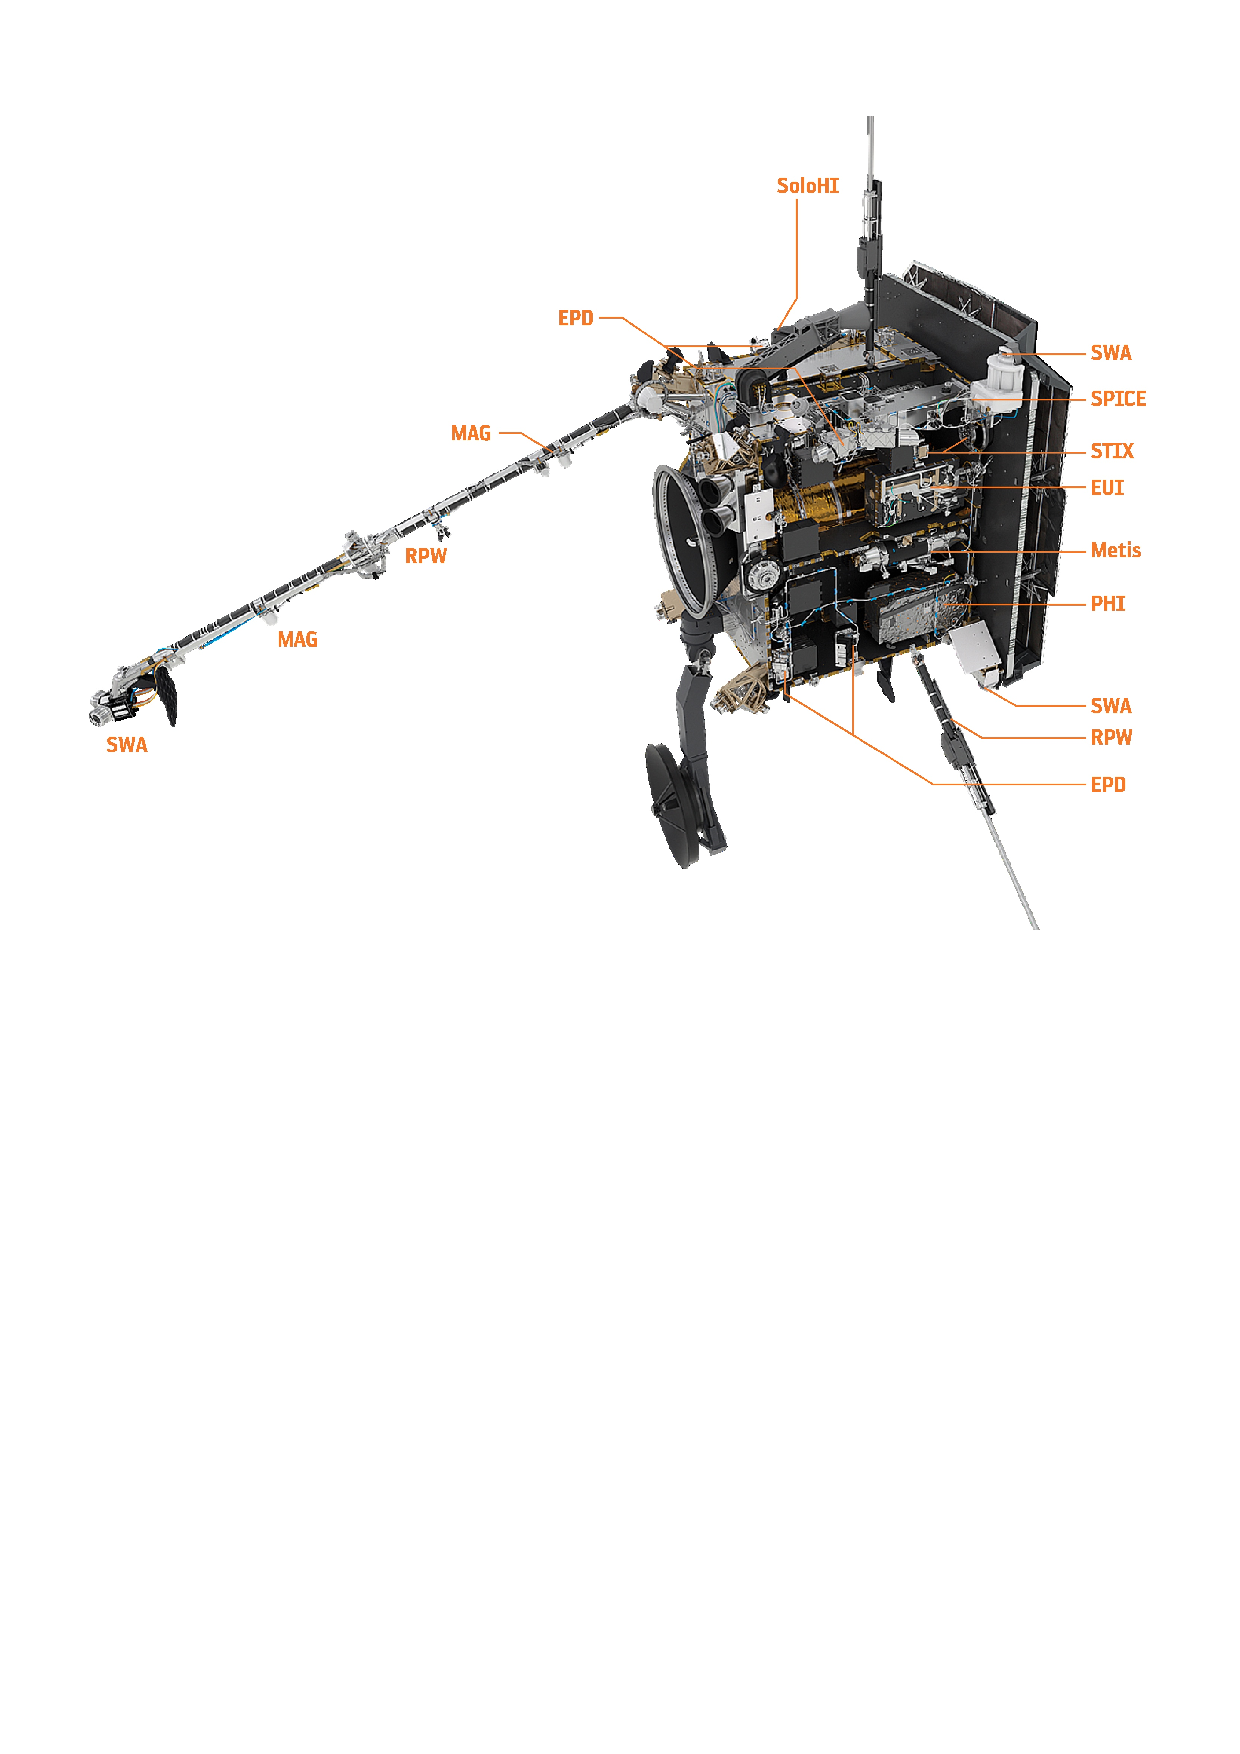
\includegraphics[width=1\linewidth]{figures/instruments.pdf}
    \caption{An image of Solar Orbiter with the -Y side panel removed to indicate the locations of onboard scientific instruments\cite{muller2020}. The boom is shown on the left-hand side of the image. Starting from the tip of the boom, in order of proximity to the spacecraft bus, the indicated instruments are SWA-EAS, MAG-OBS, RPW-SCM, and MAG-IBS\cite{horbury2020}\cite{maksimovic2020}. At the bottom right of the image is SWA-PAS, and at the top right is SWA-HIS\cite{owen2020}. }
    \caption*{Image Source: Müller et al\cite{muller2020}}
    \label{fig: instruments}
\end{figure}
\\

The overarching science objective of the Solar Orbiter mission is “How does the Sun create and control the Heliosphere – and why does solar activity change with time?”\cite{muller2020}. In service of this objective, the Solar Orbiter spacecraft carries a payload of scientific instrumentation along an inclined, eccentric solar orbit taking it to a perihelion of 0.28AU (\(\sim60\) solar radii), and up to 18\degree\ out of the ecliptic plane (extended mission phase may allow up to 30\degree). While the results from other heliophysics missions, including SOHO\cite{domingo1995}, HINODE\cite{kosugi2007}, STEREO\cite{kaiser2008}, and the Parker Solar Probe\cite{fox2016} have allowed the scientific community to make great strides towards answering similar questions to Solar Orbiter's overarching science objective, some gaps remain in our understanding of the inner heliosphere and the Sun's poles\cite{muller2020}. Solar Orbiter aims to fill those gaps.
\\

To that end, Solar Orbiter's instrumentation payload consists of a suite of remote sensing telescopes for purposes including solar wind and photospheric imaging and spectroscopy, as well as a suite of in-situ instrumentation for purposes including solar wind particle mass spectrometry and magnetic field sensing. These instruments are arranged around the spacecraft as illustrated in Figure \ref{fig: instruments}. Of particular interest to this project are the interactions between two of these in-situ instruments: The first is the Solar Wind Analyser Electron Analyser System (SWA-EAS or simply EAS); a sensor in the Solar Orbiter Solar Wind Analyser (SWA) suite of particle detectors. The second is the Solar Orbiter Magnetometer (MAG).

\section{SWA-EAS}

The Solar Wind Analyser suite comprises three in-situ particle sensors, each of which uses the well-established \q{top hat} electrostatic analyser design\cite{collinson2010}\cite{owen2020} to map incoming particles and their respective velocities/energies across each detector's field of view. The resulting maps allow the determination of the 3D \q{velocity distribution functions} (VDFs) for the particles within a given energy range over the measurement period. The three SWA sensors are: 

\begin{enumerate}
    \item The Heavy Ion Sensor (SWA-HIS or HIS), which produces VDFs for alpha particles and heavier ions in the solar wind to determine their relative charge states and abundances, not only at thermal energies, but also at \q{suprathermal} energies above the solar wind bulk speed\cite{mason2023}.
    \item The Proton-Alpha Sensor (SWA-PAS or PAS), which produces VDFs for solar wind protons and alpha particles, mainly at thermal energies.
    \item The Electron Analyser System, which produces VDFs for solar wind electrons at thermal and suprathermal energies.
\end{enumerate}

Working in concert, these sensors provide important data about local solar wind plasma to answer some of Solar Orbiter's more specific science questions, such as \q{What are the source regions of the solar wind and heliospheric magnetic field?}, \q{How do coronal mass ejections (CMEs) evolve through the corona and inner heliosphere?} and \q{How and where are energetic particles accelerated at the Sun?}\cite{owen2020}. Of the three SWA sensors, this project is most concerned with EAS. 
\\

\begin{figure}[h!]
    \centering
    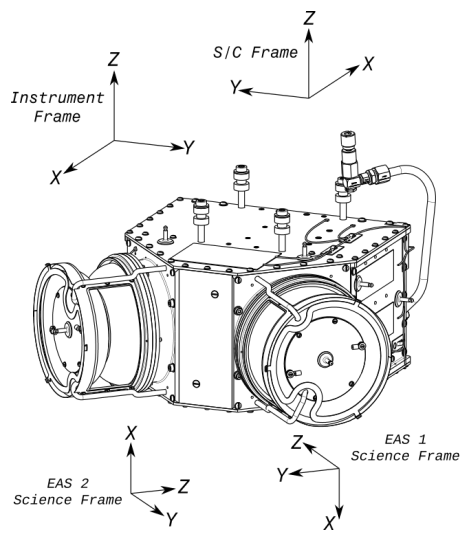
\includegraphics[width=0.75\linewidth]{figures/SWA-EA Sensor Heads.png}
    \caption{An annotated schematic depicting SWA-EAS as it appears on the end of the Solar Orbiter instrument boom (see Figure \ref{fig: instruments}), along with the axes of a few salient reference frames\cite{owen2021}. The spacecraft bus is towards the +X direction in the S/C (\q{spacecraft}) frame. The EAS1 sensor head (right) and the EAS2 sensor head (left) can be seen attached to a rectilinear electronics box.}
    \caption*{Image Source: Owen et al\cite{owen2021}}
    \label{fig: EAS schematic}
\end{figure}

EAS consists of two electrostatic analysers that inherit several aspects of their design from previous instruments such as the Cassini Plasma Spectrometer (CAPS) Electron Spectrometer (ELS)\cite{young2004}, the Mars Atmospheric and Volatile EvolutioN (MAVEN) Solar Wind Electron Analyser (SWEA)\cite{mitchell2016}, and the Cluster Plasma Electron And Current Experiment (PEACE)\cite{johnstone1997}. The two analysers, also called the \q{heads} of the instrument\cite{owen2021}, are orthogonal to each other as shown in Figure \ref{fig: EAS schematic}. Unlike HIS and PAS, which can afford relatively narrow, Sun-pointing fields of view (FOV) of 33° to +66° × ±20° and 24° to +42° × ±22.5° respectively, the EAS sensor heads each observe 360\degree\ of azimuth and ±45\degree\ of elevation in their respective reference frames (see \q{EAS 1/2 Science Frame} in Figure \ref{fig: EAS schematic}), theoretically covering more than the sky's full 4\(\pi\) steradians between them, where \(1.6\pi\) steradians are covered by the overlap between the two FOVs (see Figure \ref{fig: all bins})\cite{owen2020}. This FOV is required because, in comparison to protons and other ions, electron thermal velocities are expected to be much higher than the solar wind plasma bulk velocities. As a result, while protons and other ions are expected to enter their respective sensor primarily from the Sun-facing direction, electrons are expected to enter EAS more isotropically\cite{owen2020}. In reality, some of the EAS FOV is always obstructed by a set of support pillars and a shielding grid (to avoid spacecraft engine exhaust contamination) around each head, as well as the Solar Orbiter bus high-gain antenna and solar arrays\cite{owen2020}\cite{owen2021}\cite{dickson2024}. To minimise this obstruction, as well as to avoid electrostatic interference from the rest of the spacecraft,  EAS is positioned at the far end of the 4.4m Solar Orbiter instrument boom (see Figure \ref{fig: instruments})\cite{owen2020}\cite{olaskoaga2017}.
\\

\begin{figure}[h!]
    \centering
    \centerfloat
    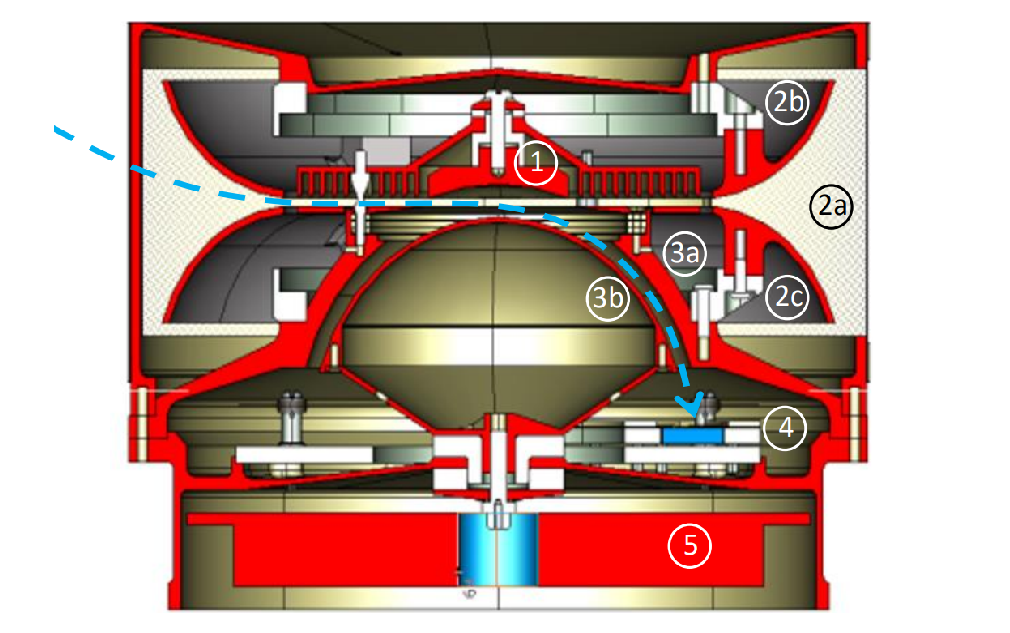
\includegraphics[width=0.85\linewidth]{figures/eas_cross-section.png}
    \caption{A diagram showing a cross-section of an EAS sensor head with an example electron trajectory illustrated in blue, and the following annotated subsystems\cite{owen2020}: (1) “top-cap” anode for controlling the geometric factor; (2) (a) sensor shielding grid; (2) (b,c) deflector electrodes for elevation selection; (3) (a,b) hemispherical electrodes for energy selection; (4) MCP subsystem; (5) charge amplifier integrated circuit.}
    \caption*{Image Source: Owen et al\cite{owen2020}}
    \label{fig: EAS cross-section}
\end{figure}

Ignoring obstructions, solar wind electrons can enter each sensor head from any elevation and azimuthal angle in its field of view. As they do so, the electrons fly through an electric field generated by a pair of deflector electrodes at the entrance of the head (subsystems 2b and 2c in Figure \ref{fig: EAS cross-section}). The electrodes are charged with positive voltages such that only incoming electrons from a narrow, selected range of elevation angles can continue through the sensor head. Electrons with elevations outside of this range will collide with the sensor walls and go undetected. This range corresponds to a single elevation angle bin. Electrons within the selected elevation range subsequently fly through a pair of hemispherical electrodes (subsystems 3a and 3b in Figure \ref{fig: EAS cross-section}). These electrodes create an electric field that only allows electrons within a narrow, selected range of velocities/energies to continue to the detector proper, filtering the electron population again. This range corresponds to a single energy bin. If an electron passes through these electron optics, then its trajectory ends when it impinges on a segment of an annular microchannel plate (MCP) corresponding to its azimuthal angle (subsystem 4 in Figure \ref{fig: EAS cross-section}). As a result, the incoming electron induces the emission of \(2\times10^{6}-5\times10^{6}\) secondary electrons which collect at the MCP anode, resulting in a characteristic voltage pulse that triggers a detection\cite{owen2020}.
\\

During EAS operation, the deflector electrodes sweep through up to 16 elevation bins, sequentially, in the range of ±45\degree. The elevation bins are unequally sized according to a\footnote{SWA-EAS has used different elevation bin tables at different times over the course of the Solar Orbiter mission. Due to an error in the EAS data acquisition pipeline discovered during this project, this table has occasionally been incorrect (see Section \ref{sim steering}).} table of voltages aboard Solar Orbiter, which is designed to account for increasing angular resolution at increasing deflection angles, with bin widths varying from \(\sim2\degree\) to \(\sim10\degree\). For each elevation bin, the hemispherical electrodes sweep through up to 64 logarithmically-spaced energy bins, sequentially, in the range \([\sim1\textrm{eV},\sim5\textrm{keV}]\). The full range of 0-360\degree\ of azimuth is split into 32 equally-spaced azimuthal bins, all of which are sampled simultaneously for each combination of elevation and energy. The result is a distribution of solar wind electron energies per solid angle; an electron VDF.
\\

\section{MAG}
The Solar Orbiter magnetometer consists of two three-axis fluxgate magnetometers located on the Solar Orbiter instrument boom. The inboard sensor (MAG-IBS) and outboard sensor (MAG-OBS) respectively (see Figure \ref{fig: instruments}).  The two sensors are at different positions along the boom to minimise the risk of magnetic contamination by the rest of Solar Orbiter both by distance attenuation and by subtracting the effect of Solar Orbiter through magnetic gradiometry. The design of MAG borrows heavily from that of previous magnetometers flown on the Cassini\cite{dougherty2004} and Double Star\cite{carr2005}, missions, and forms the basis for future magnetometers on missions including IMAP\cite{mccomas2018}\cite{dickson2024}. The author has previously described the operation of a fluxgate magnetometer as follows\cite{dickson2024}: 

Each magnetometer consists of two orthogonal fluxgate ring-cores (one of which is partially visible in Figure \ref{fig: magnetomato}). The fluxgate cores consist of three copper windings; One inner “drive” winding and two outer, orthogonal, “sense” windings. The inner “drive” winding is wound around a ring of magnetically-permeable material which it drives into successive states of oppositely-polarised magnetic saturation at the “drive frequency” through magnetic induction. In an environment with no external magnetic field, the magnetic field induced in one half of the ring is designed to perfectly counteract the antisymmetric field induced in the opposite half, resulting in zero magnetic field in the ring overall. However, if an external magnetic field is present and oriented along the plane of the ring, then the drive winding will drive the ring core into magnetic saturation more quickly in the direction parallel to the external magnetic field and more slowly in the direction antiparallel to the external magnetic field. The effect of such an external magnetic field is to temporarily break the symmetry of the induced magnetic field in the ring core, causing a pulse of magnetic flux density which repeats at twice the drive frequency. These pulses induce voltages in the outer sense windings from which a 2D external magnetic field vector can be recovered. With two orthogonal ring-cores, each fluxgate magnetometer can recover an external magnetic field vector in full 3D\cite{horbury2020}\cite{dickson2024}. 
\\

\begin{figure}[h!]
    \centering
    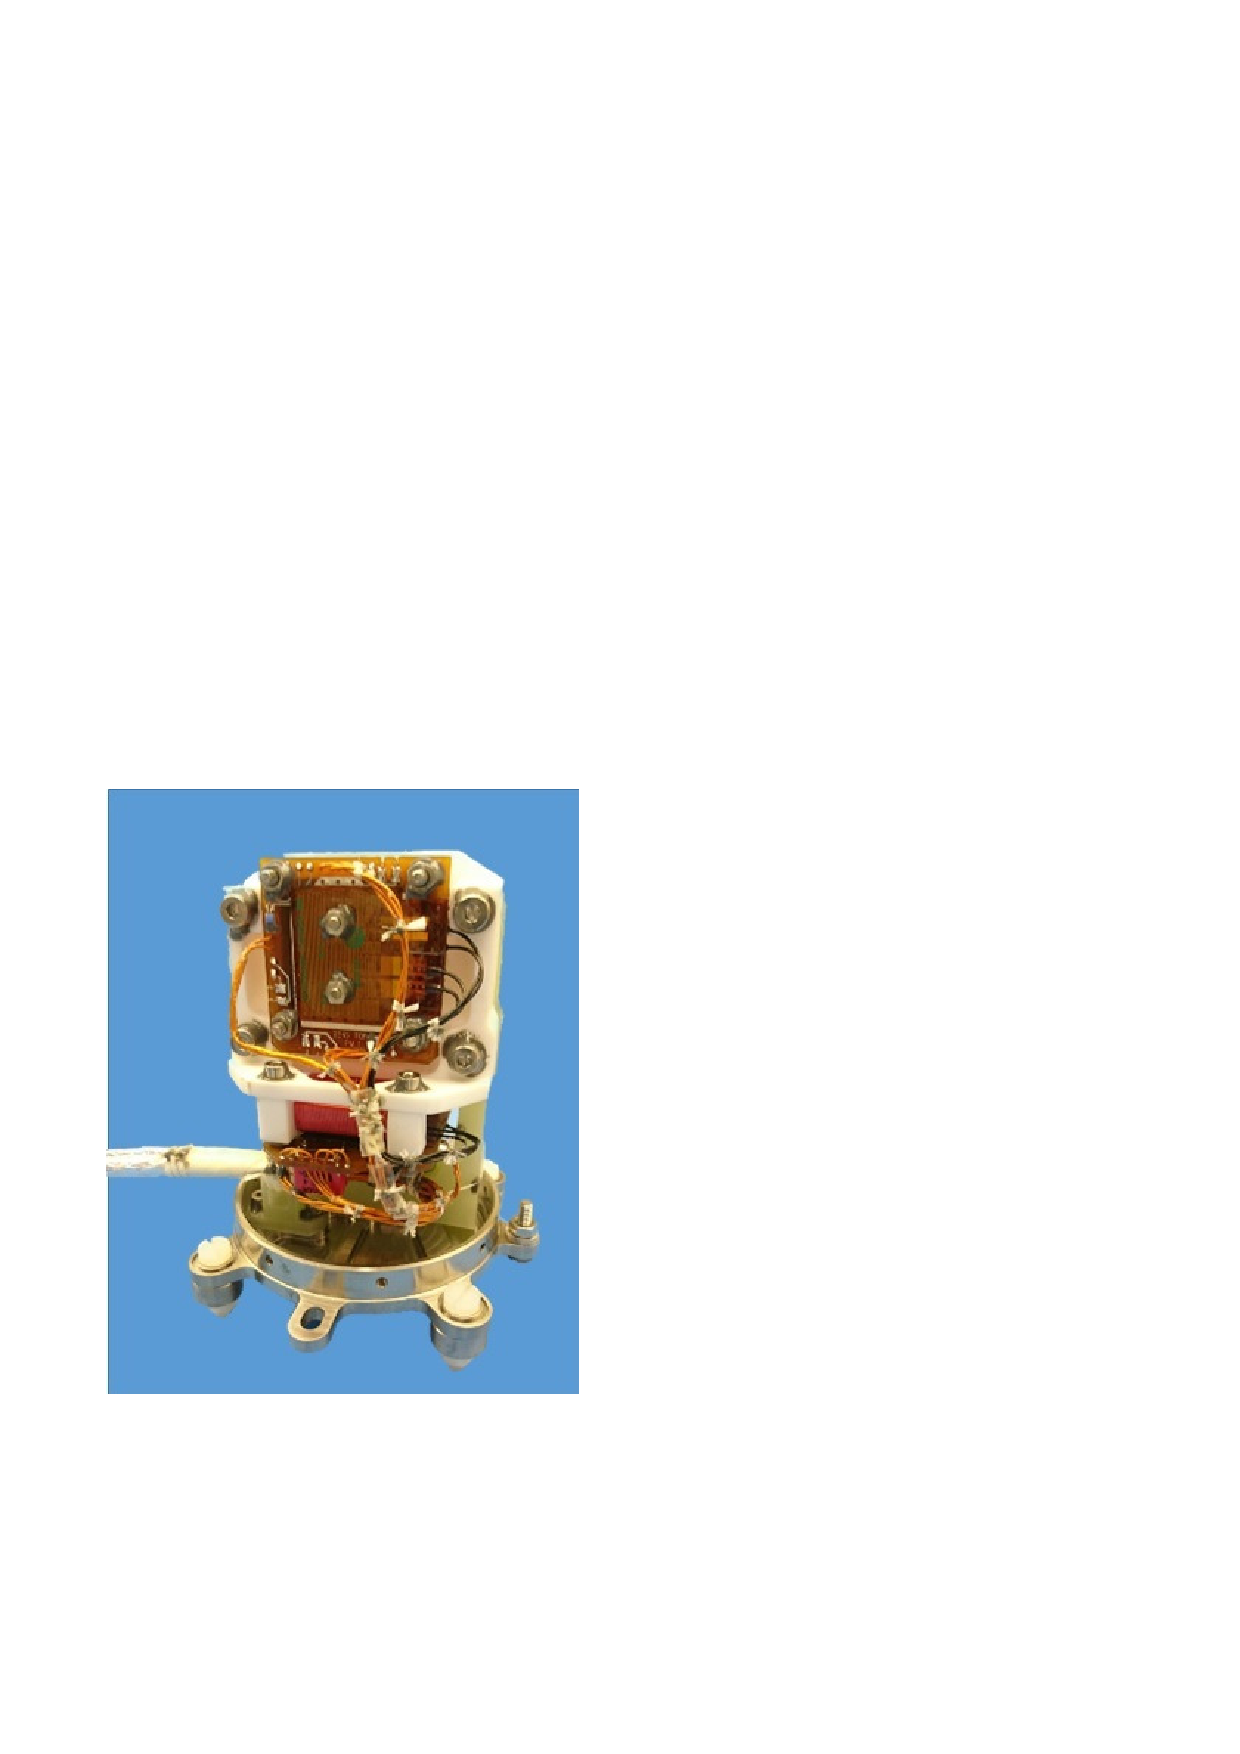
\includegraphics[width=0.5\linewidth]{figures/magnetomato.pdf}
    \caption{An image of one of the Solar Orbiter fluxgate magnetometer sensors as seen in the lab with its protective radiation shield removed\cite{horbury2020}. One ring core with its bright red outermost sense winding can be seen mounted on the underside of a white, ceramic bracket. The other core is unseen, mounted on the other side.}
    \caption*{Image Source: Horbury et al\cite{horbury2020}}
    \label{fig: magnetomato}
\end{figure}


The measured values of the axial components of the external magnetic field vector are known to occasionally “drift” due to imperfections in the magnetometer hardware, leading to offsets that affect magnetic field vector orientation. These offsets are corrected through data processing on the ground and through occasional updates to the software aboard Solar Orbiter\cite{horbury2020}. The central issue in this project is the effect of onboard MAG data inaccuracies, including offset, on EAS pitch angle data. 

\section{EAS Pitch Angle Distributions} \label{EAS PAD}
A particle's pitch angle, often denoted \(\alpha\), is the angle between the particle's velocity vector \(v\) and the local magnetic field vector \(B\). \(\alpha\) is given by:

\begin{equation} \label{eq: pitch angle}
    \alpha=\arctan{\frac{v_\perp}{v_\parallel}}
\end{equation}

where \(v_\parallel\) and \(v_\perp\) are the particle's velocity components parallel and perpendicular to \(B\) respectively\cite{pilipp1987}. Analysis of electron pitch angle distributions (PADs) has revealed distinct electron populations in the solar wind. Some populations have a tendency to collide amongst themselves, resulting in a \q{thermal} distribution with mainly isotropic pitch angles that  can be modeled, to within a close approximation, by a Maxwell-Boltzmann distribution. These represent the \q{bulk} of the electron plasma. Other populations are more anisotropic, forming narrow electron beams with pitch angles that may be field-aligned, making up the so-called  electron \q{strahl}. These anisotropic electrons tend to collide less frequently, so their trajectories are less uniformly distributed\cite{pilipp1987}\cite{marsch2006}.
\\

\begin{figure}[h!]
    \centering
    \centerfloat
    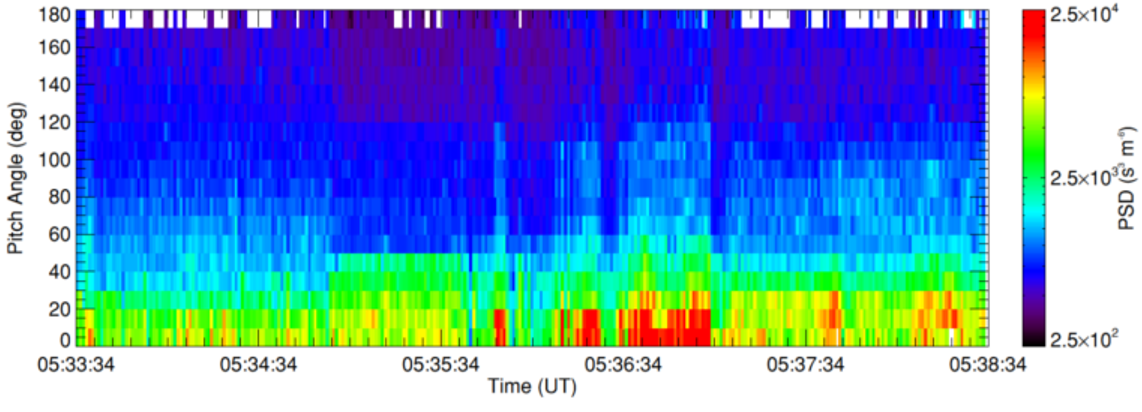
\includegraphics[width=1.1\linewidth]{figures/PADexample.png}
    \caption{Pitch angle data recorded by Solar Orbiter SWA-EAS in Burst Mode over 5 minutes on 26th June 2020\cite{owen2021}. Electron counts are plotted as a PSD. Time is plotted in Universal Time. Electron pitch angle is plotted in degrees.}
    \caption*{Image Source: Owen et al\cite{owen2021}}
    \label{fig: PAD example}
\end{figure}

An example PAD generated using Solar Orbiter SWA-EAS data is shown in Figure \ref{fig: PAD example} for a 5-minute period starting at 05:33:34 UT on 24th June 2020\cite{owen2021}. Shown here is the phase space density, or concentration, of strahl electrons with energies \(>70\)eV. The concentration is presented in terms of power spectral density (PSD) in colours from black (fewest electrons) to red (most electrons)\footnote{White pitch angle bins on this plot represent missing data, relating to each PAD's completeness score, which will be important in Section \ref{completeness}.}. A different PAD is plotted at every 1/8th-second time step (corresponding to EAS Burst Mode; see below). Notice that, for each time step, only pitch angles are shown from 0\degree\ to 180\degree\. It may seem that a full map of the sky would be required to fully capture electron concentrations at different phase angles about the local magnetic field at a given pitch angle, implying \textit{two} angles in spherical coordinates for every time step. However, near this time resolution, it is expected that any instantaneous in-homogeneities in electron concentration at different gyrophase angles about the local magnetic field will disappear too quickly to discern, such that the concentration at all phase angles for a given pitch angle can be assumed to be uniform; in a state of so-called \q{gyrotropy}\cite{owen2021}. This is expected to be a safe assumption at this timescale\cite{vocks2012}\cite{spinnangr2022}\cite{owen2021}. This can be understood because the expected electron gyroperiod in the solar wind at \(\sim\)1AU is much shorter than the 1/8th-second timescale. Assuming magnetic field strength \(B\approx1\textrm{nT}\), then the electron gyrofrequency \(\omega_{e}\) is given by:

\begin{equation} \label{eq: gyrofreq}
    \omega_{e}=\frac{eB}{m_{e}}=\frac{e\times10^{-9}}{m_{e}}\approx176\textrm{ rad/s}
\end{equation}

where \(m_{e}\) is the electron mass. The corresponding gyration frequency is therefore \(\omega/2\pi\approx28.0\textrm{/s}>>8\textrm{/s}\). Therefore, if this is a realistic estimate, then over a single 1/8th-second measurement, most electron agyrotropy is expected to be thoroughly averaged and rendered indiscernible. Lu et al 2020 has similarly supported the assumption of  gyrotropy when using 1/4th-second time steps in 2D particle-in-cell simulations of magnetic reconnection at Earth, on the basis that the local electron gyroradius should be comparable in size to the local plasma ion skin depth - should this be analogous to the EAS environment with the solar wind's plasma parameters to within an order of magnitude, then the assumption of gyrotropy for EAS is expected to be safe\cite{lu2020}\cite{lu2019}.
\\

The PAD in Figure \ref{fig: PAD example} was taken while EAS was operating in \q{Burst Mode}, which differs from the more typical \q{Normal Mode} in that it generates PADs \(\sim8\times\) faster. A description of Normal Mode and Burst Mode PAD determination follows.



\subsection{EAS Normal Mode} \label{EAS Normal Mode}

Most EAS data are collected in normal mode, where all 64 energy bins, 16 elevation bins, and 32 azimuth bins are sampled, yielding as close to a full-sky VDF as possible. The 32 azimuth bins are sampled simultaneously. Sampling a single energy bin for a single elevation bin takes \(\sim0.96\)ms\cite{owen2021}. Therefore, cycling through all energy and elevation bins in sequence takes \(64\times16\times0.96\textrm{ms}=0.983\textrm{s}\approx1\textrm{s}\), yielding Normal Mode data at a data rate of \(\sim1\)Hz\cite{owen2021}. The pipeline involved in acquiring a VDF and a subsequent PAD in Normal Mode can be summarised as follows\cite{owen2020}:

\begin{enumerate}
    \item Acquire a full-sky EAS VDF with 64 energy bins \(\times\) 16 elevation bin \(\times\) 32 azimuth bins at 1Hz,
    \item Acquire a MAG vector at 1Hz,
    \item Downlink EAS VDF and MAG vector to ground,
    \item Post-process MAG vector on ground, applying any necessary corrections,
    \item Combine EAS VDF and MAG vector to yield a PAD.
\end{enumerate}

For a more detailed description, consider Figure \ref{fig: all bins}. This figure shows the combined elevation and azimuth bin \q{pixels} available to each EAS sensor head (EAS1 in blue and EAS2 in red) projected on to a map of the full sky in spherical, spacecraft reference frame (SRF) coordinates where [0,0] points directly away from the Sun, and +90\degree\ elevation points out of the ecliptic plane. This amounts to a total of \(16\time32=512\) pixels per head. In normal mode, an EAS head first samples electrons from all of the pixels in its FOV. Meanwhile, MAG samples the local 3D magnetic field vector in its own Burst Mode (128Hz) or Normal Mode (8Hz)\cite{horbury2020}. Now, consider Figure \ref{fig: normal - full contours}, where a magnetic field vector from the same period as the 1s PAD is superimposed onto a projection of the EAS1 bins in SRF coordinates. Here, the green diamond represents the vector parallel to the magnetic field (i.e. the B-vector itself), and the green square represents the antiparallel vector. Surrounding the parallel vector are various contours of constant pitch angle at every 15\degree\ in the range \([0\degree,180\degree]\). To aid explanation, let the vectors in Figure \ref{fig: normal - full contours} represent the ground magnetic field post-processing\footnote{In reality, this vector was taken from data from the archive corresponding to the unprocessed magnetic field transmitted over the S20 data link in EAS Burst Mode (see Section \ref{EAS Burst Mode}). In this case, it is only treated as an analogy for the ground magnetic field.}. In this case, wherever an EAS pixel is crossed by a pitch angle contour, that pixel has sampled electrons with the contour's pitch angle. Calculating the pitch angle for every pixel in the 3D VDF allows a 2D PAD to be constructed for every azimuthal bin, each of which corresponds to a range of gyrophase angles. By combining samples from all the azimuthal bins in post-processing (this is harmless under gyrotropy), the gyrophase dimension is collapsed, yielding a single, 2D PAD for the 3D VDF.
\\

Even with compression, the volume of data implied by a full-sky, 3D VDF in Normal Mode has significant implications for the SWA telemetry budget, limiting full-cadence (1s/sample or 1Hz) data downlink to a 5-minute period per day. Instead, the SWA Data Processing Unit (SWA-DPU) typically downlinks moments of full VDFs at a cadence of 4s/sample, and full VDFs are limited to 10s/sample or 100s/sample cadences when downlinked. The limited telelmetry budget places even more constraints on what is already a relatively low cadence for measurements of solar wind electron dynamics (baseline of 1s/sample), motivating the design of a faster and less data-intensive method of operation; EAS Burst Mode.

\begin{figure}[h!]
    \centering
    \centerfloat
    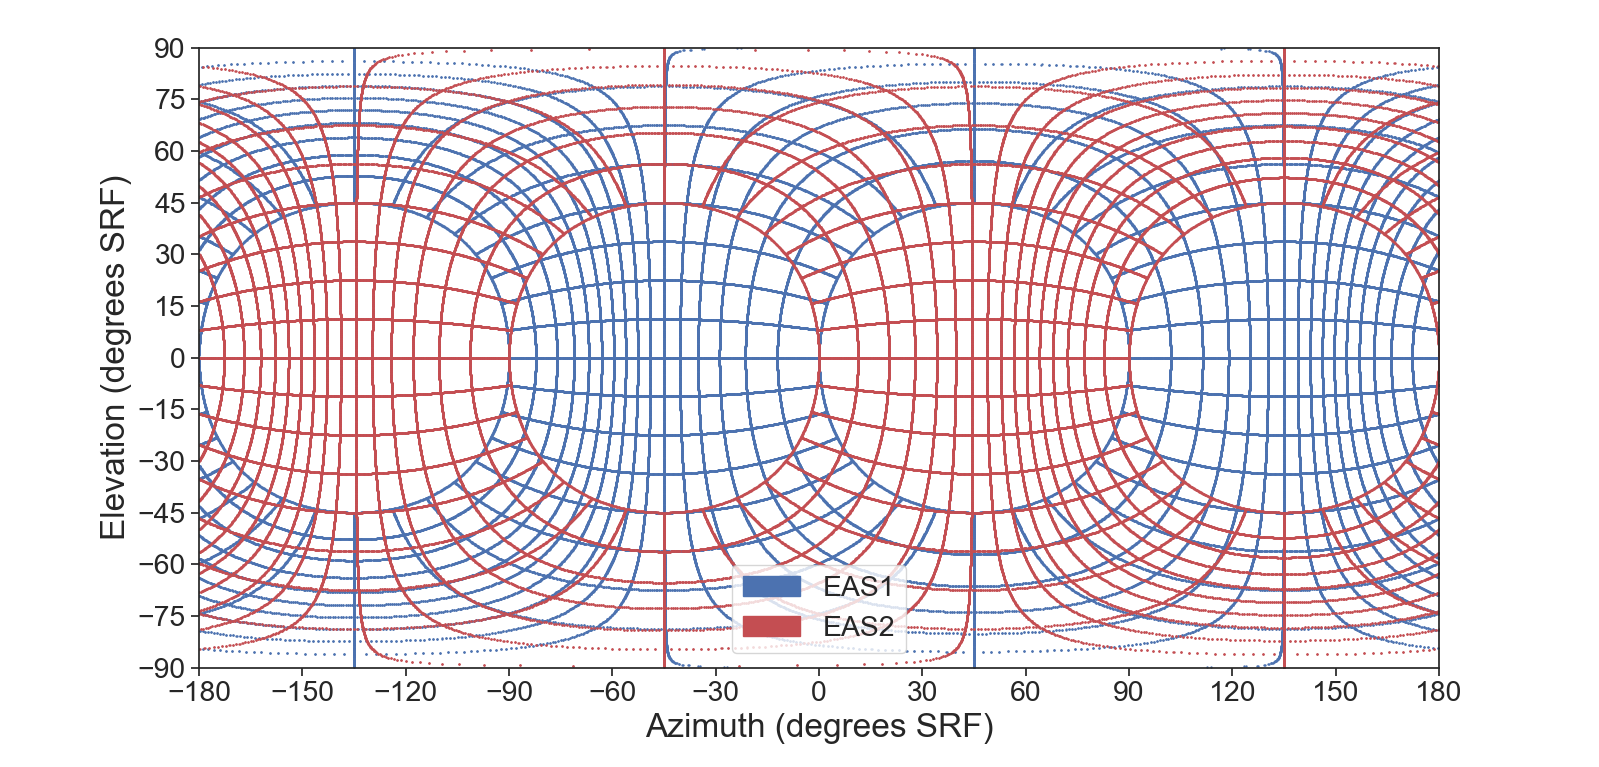
\includegraphics[width=1.2\linewidth]{figures/all bins.png}
    \caption{A plot  of EAS1 (blue) and EAS2 (red) elevation and azimuth bins projected onto the sky in spherical spacecraft reference frame (SRF) coordinates. Note that \q{elevation} and \q{azimuth} as labelled in the axes refer to the coordinates in SRF; \textit{not} the elevation/azimuth in the sensor head frames (e.g. Figure \ref{fig: EAS schematic}). Note also that between EAS1 and EAS2, it is possible to cover the entire sky with some overlap.}
    \caption*{Image Source: Author's own work}
    \label{fig: all bins}
\end{figure}

\begin{figure}[h!]
    \centering
    \centerfloat
    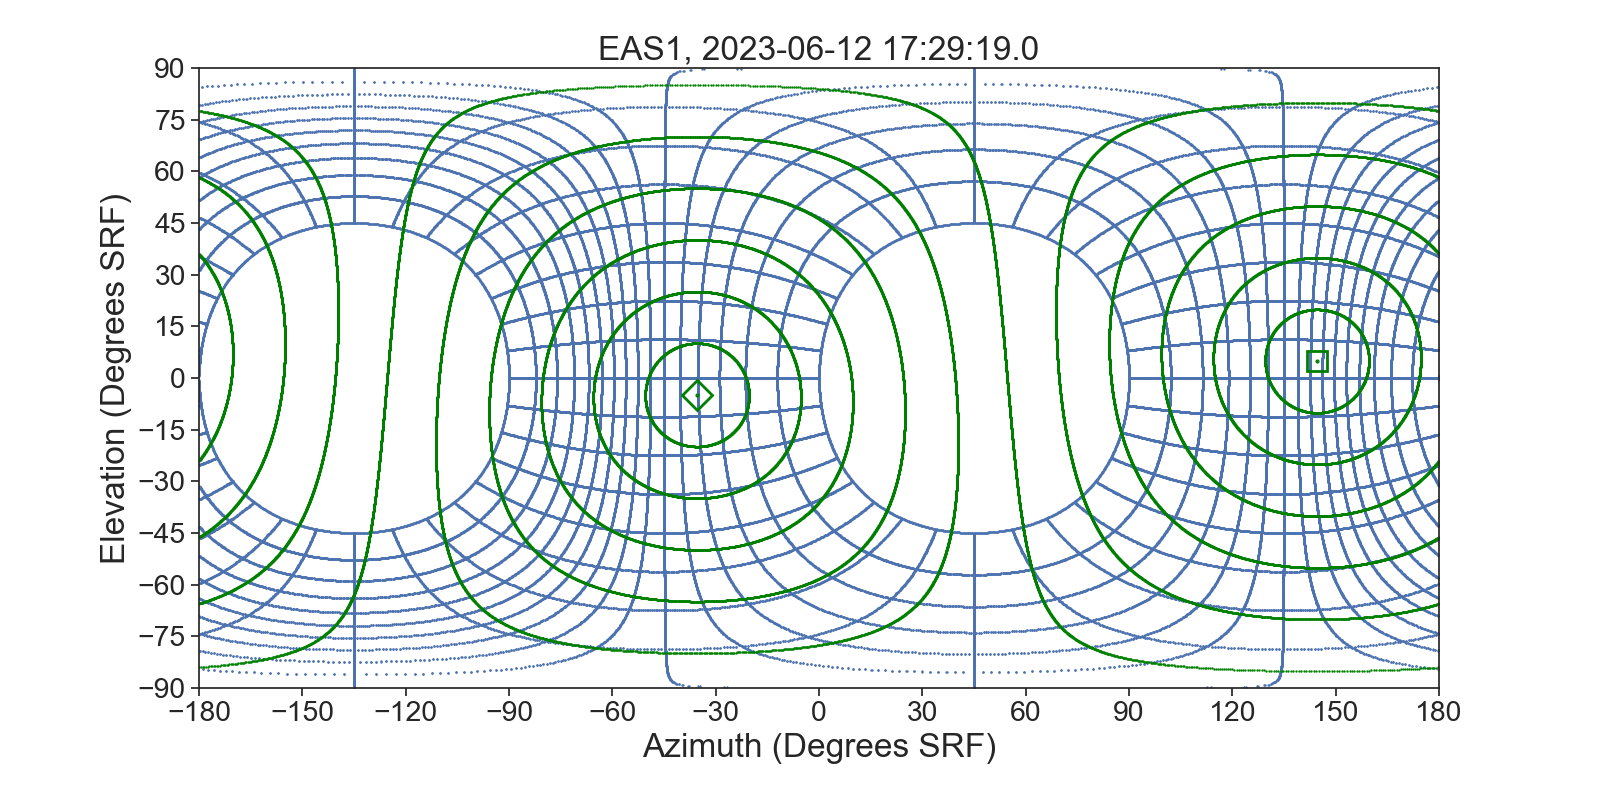
\includegraphics[width=1.2\linewidth]{figures/fullcontours_justeas_noselection.png}
    \caption{Another plot of projected EAS1 elevation and azimuth bins in SRF overlaid with a magnetic field vector from MAG. The point parallel to the vector is indicated by the green diamond, and the point anti-parallel to the vector is indicated by the green square. The green contours represent pitch angles in 15\degree increments from 15\degree to 165\degree. MAG vector data are taken from the Solar Orbiter Archive, from a period of data collection on 12th June 2023. }
    \caption*{Image Source: Author's own work}
    \label{fig: normal - full contours}
\end{figure}


\newpage
\subsection{EAS Burst Mode} \label{EAS Burst Mode}

EAS Burst Mode data are typically collected over periods of \(\sim5-15\)minutes, once per day. Compared to Normal Mode at full cadence, full Burst Mode PADs can be acquired after sampling only 2 of the 16 elevation bins in the sky, resulting in a theoretical \(8\times\) improvement in sample cadence (8Hz at \(\sim0.125\)s/sample). Compared to other typical Normal Mode cadences of 4s/sample, 10s/sample, or 100s/sample, the improvement can be as good as \(32\times\), \(80\times\), or \(800\times\) respectively. The Burst Mode PAD pipeline can be summarised as follows\cite{owen2021}:

\begin{enumerate}
    \item Acquire a MAG vector at 8Hz,
    \item Transmit the MAG vector directly to EAS via the onboard \q{S20} data link,
    \item Select the EAS head that has the MAG vector closest to the center of its FOV,
    \item For that head, select the \textbf{2} elevation bins that contain the parallel and antiparallel MAG vector in their respective FOVs,
    \item Acquire a partial-sky VDF with 64 energy bins \(\times\) 2 selected elevation bins \(\times\) 32 azimuth bins at 8Hz,
    \item Downlink EAS VDF to ground,
    \item Re-bin EAS VDF on ground, yielding a full PAD.
\end{enumerate}

\begin{figure}
    \centering
    \centerfloat
    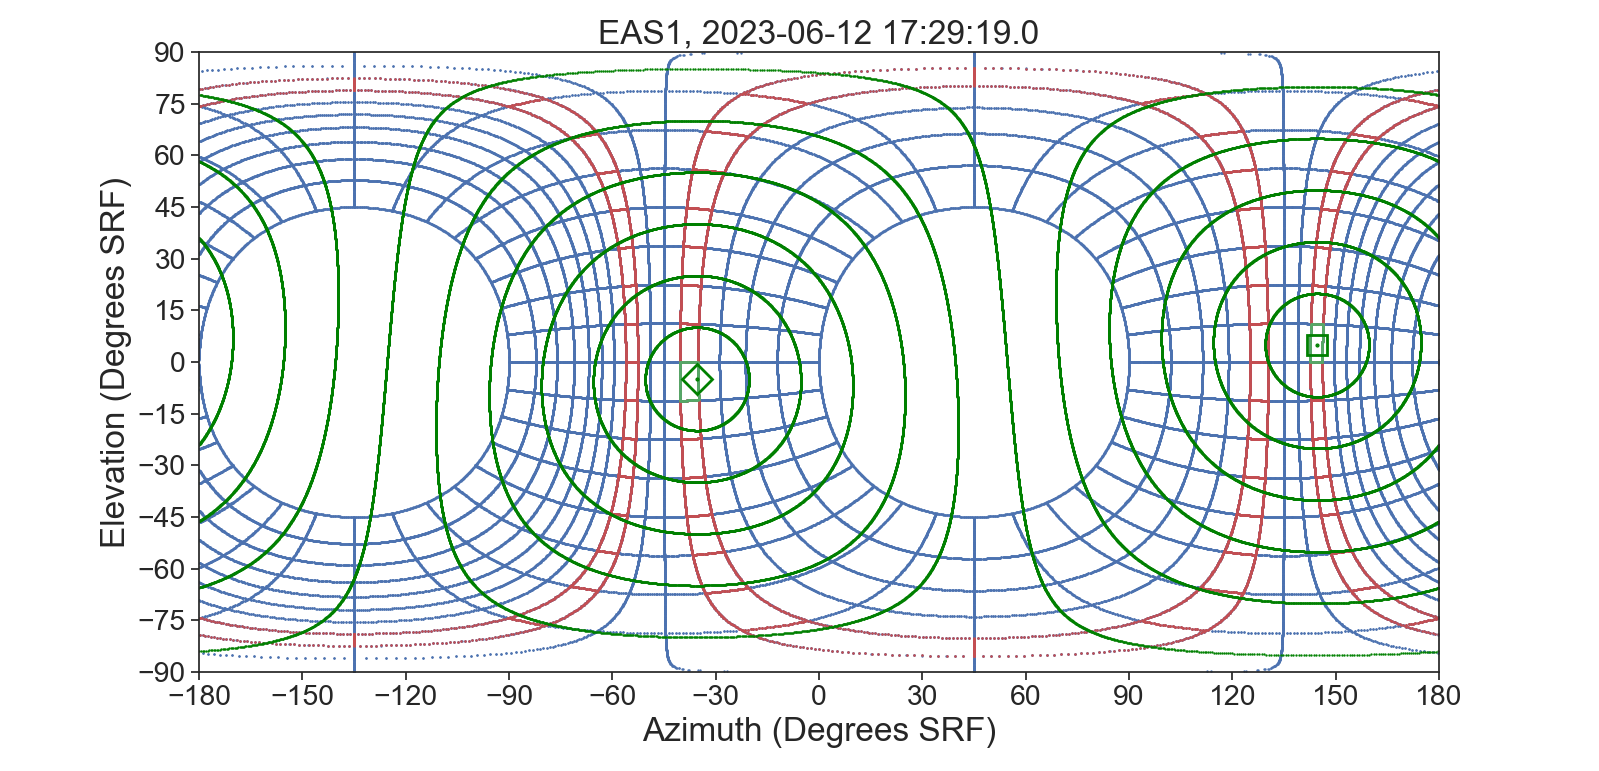
\includegraphics[width=1.2\linewidth]{figures/fullcontours_justeas_yesselection.png}
    \caption{A similar plot to Figure \ref{fig: normal - full contours}. Additionally, the bands of EAS1 elevation bins containing the parallel and antiparallel magnetic field vectors are highlighted in red, and the elevation and azimuth pixels containing the same vectors are highlighted in green. MAG vector data are taken from the Solar Orbiter Archive, from a period of data collection on 12th June 2023. }
    \caption*{Image Source: Author's own work}
    \label{fig: normal - full contours + selection}
\end{figure}

For a more detailed description, consider Figure \ref{fig: normal - full contours + selection}. This figure shows the same bins, vectors, and pitch angle contours as Figure \ref{fig: normal - full contours}, but the bands of elevation bins containing the parallel and antiparallel magnetic field vectors are highlighted in red, and the pixels containing the parallel and antiparallel magnetic field vectors are highlighted in green. Note that each elevation band is separated into azimuthal bins. Within the elevation band containing the parallel vector, as angular distance increases from the azimuthal bin/pixel containing the vector, successive azimuthal bins are crossed by higher and higher pitch angles, culminating in an angle \(\alpha\geq90\degree\). Conversely, as angular distance increases from the azimuthal bin containing the antiparallel magnetic field vector, successive azimuthal bins are crossed by lower and lower pitch angles, culminating in an angle \(\alpha\leq90\degree\). For the sensor head containing the magnetic field vector in its FOV, the geometry of the sensor heads guarantees that this is always true\cite{owen2021}; the two opposite sides of a hypothetical elevation bin at 0\degree\ elevation would reach a maximum of \(\sim180\degree\) apart, and the opposite sides of an elevation bin at \(\pm45\degree\) would reach a minimum of \(\sim90\degree\) apart. Therefore, by \q{steering} EAS to sample each azimuthal bin across only the two highlighted elevation bands, it is possible to sample electrons with a full range of 0\degree-180\degree\ pitch angles. With the assumption of gyrotropy, this represents a full PAD (e.g. Figure \ref{fig: PAD example}). Since the 32 azimuth bins at each elevation are sampled simultaneously, this costs no additional time, resulting in an eight-fold sample time reduction.
\\

To sample only the elevation bins containing the parallel and antiparallel magnetic field vector, EAS must first be told the orientation of the magnetic field. On Solar Orbiter, this is communicated via the \q{S20 inter-instrument communications link} which is transmitted by the MAG Instrument Control Unit (MAG-ICU) and received by the SWA-DPU\cite{owen2021}\cite{owen2020}\cite{horbury2020}. Once received, SWA-DPU must select the EAS head that has the magnetic field closest to the center of its FOV, which is equivalent to finding the smallest angle between the vector and the sensor head aperture center-plane\cite{owen2021}.
\\

While Burst Mode boasts far-superior time resolution, it is also vulnerable to errors that Normal Mode avoids. By virtue of the fact that Burst Mode uses MAG data transmitted directly over the S20 data link, it therefore also does not benefit from post-processing of MAG data on the ground. Errors that may result in a discrepancy between the vectors used to \q{steer} EAS and the \q{more-correct} ground vectors include: 
\begin{itemize}
    \item Un-calibrated offset drift in MAG measurement axes, which may be more significant during the period leading up to a routine calibration update\cite{owen2021}\cite{horbury2020}.
    \item Data latency in the S20 inter-instrument link itself, which may be inherent and/or exaggerated  by periods of heavy data traffic\cite{owen2021}.
\end{itemize}

When errors like these cause EAS to select incorrect elevation and azimuth bins in Burst Mode, this can lead to missing and mislabelled PAD data. The next chapter describes the methods applied to analyse the impact of these and other errors on Burst Mode PAD accuracy and completeness, and to encapsulate some of that impact in the form of a \q{completeness score}.


\chapter{Methods}
\label{chapterlabel2}

To determine the accuracy and completeness of Burst Mode data collection it is useful to compare 3D magnetic field vectors used to steer EAS in Burst Mode (which will be called \q{\Beas}) to corresponding examples of the ground-calibrated and \q{true} magnetic field vectors (which will be called \q{\Bmag}).
\\

\section{Data Access} \label{data}
The online Solar Orbiter Archive (SOAR) regularly publishes science data at various processing levels from Solar Orbiter instruments, including MAG and EAS, where they can be accessed by the public\cite{soar}. Most science data, including MAG vector time series and EAS Burst Mode PADs, are published in CDF, which is a \q{Self-describing data format for the storage of scalar and multidimensional data in a platform- and discipline-independent way}\cite{cdf}. Developed by NASA Goddard Space Flight Center, CDF is an industry-standard data format used frequently in NASA/ESA projects\cite{horbury2020}. CDF files accommodate data fields for different variables including science data and associated metadata/support data, along with various tags and descriptions. The primary data and metadata in a CDF file can be previewed via the SOAR interface, and accessed/manipulated through freely available libraries built for Python and MATLAB\cite{cdf}.
\\

EAS and MAG data products are published to SOAR at various levels of usability; some are \q{raw} data directly from the instrument, and others are thoroughly processed and ready to be used in conventional, publishable research\cite{horbury2020}\cite{owen2020}\cite{zouganelis2020}. The author has previously described the data levels for EAS and MAG as follows\cite{dickson2024}:
\\

\textbf{EAS Data Levels\cite{owen2020}:}
\begin{itemize}
    \item \textbf{Level 0:} Uncalibrated CCSDS\cite{CCSDS_Standards_2022} binary data packets.
    \item \textbf{Level 1:} Uncalibrated electron count data converted to CDF in Burst Mode and Normal Mode. At this level, the MAG vectors used to steer EAS during Burst Mode (\(B_{EAS}\)) are also included.
    \item \textbf{Level 2:} Calibrated electron count data including Burst Mode PADs, but excluding \(B_{EAS}\).
    \item \textbf{Level 3:} A subset of level 2 data with additional processing.
\end{itemize}

\textbf{MAG Data Levels\cite{horbury2020}:}
\begin{itemize}
    \item \textbf{Level 0:} Uncalibrated binary data.
    \item \textbf{Level 1:} Uncalibrated time series data in nT in each MAG sensor's reference frame.
    \item \textbf{Level 2:} Calibrated time series data in radial-tangent-normal (RTN), and Spacecraft Reference Frame (SRF) coordinates, corrected for offset drift and other inaccuracies, published at various cadences including E8 normal mode (8Hz) and E128 burst mode (128Hz).
    \item \textbf{Level 3:} A subset of level 2 data with additional processing.
\end{itemize}


EAS level 1 (L1) Burst Mode CDF files are typically published at a rate between \(\sim\)5min/day and \(\sim\)15min/day. Some of these files are published to SOAR under the name \q{solo\_L1\_swa-eas-padc\_\textit{YYYYMMdd}T\textit{hhmmss}-\textit{YYYYMMdd}T\textit{hhmmss}\_V01.cdf}, and these particular files are packaged with \(B_{EAS}\) as metadata in the form of normalised vectors in the SRF frame under the variable \q{SWA\_EAS\_MagDataUsed}. 

MAG level 2 (L2) SRF CDF files, published to SOAR under \q{solo\_L2\_mag-srf-normal\_\textit{YYYYMMdd}\_V01}, contain several hour's worth of ground-calibrated 8Hz MAG data per day (i.e. \(B_{MAG}\)), all in the same reference frame as \(B_{EAS}\) at the time of publishing (SRF), under the variable \q{B\_SRF}.
\\

The desired CDFs were downloaded and manipulated using Python scripts with the \textit{pycdf} package in the Spacepy library. Spacepy is \q{a package for Python, targeted at the space sciences, that aims to make basic data analysis, modeling and visualization easier}\cite{niehof2022spacepy}. Pycdf allows individual CDF data fields to easily be referenced by name and converted to \textit{numpy} arrays as required\cite{harris2020numpy}.

\section{Time Axis Cropping}
\Beas\ and \Bmag\ can be plotted together at 8Hz to yield an initial estimate of the discrepancies between them, but their recent, respective time series are uploaded to SOAR with very different durations (typically 5-15 minutes vs several hours respectively). This makes it difficult to compare one time series to the other numerically using Python, unless the longer time series is first cropped.  Several algorithms were implemented to crop magnetic field time series. Initial attempts involved simply cropping the start and end of the longer series  (\(B_{MAG}\)) to the shorter series (\(B_{EAS}\)). While this worked for some EAS CDFs (e.g. solo\_L1\_swa-eas-padc\_20231105T172733-20231105T174232\_V01.cdf, lasting 15mins, and solo\_L1\_swa-eas-padc\_20230831T172734-20230831T173233\_V01.cdf, lasting 5mins), this could not be generalised to some older EAS CDFs which combined multiple Burst Mode periods totalling 1hr or more of duration (e.g. solo\_L1\_swa-eas-padc\_20200624T053335-20200624T063334\_V01.cdf, lasting 1hr, and solo\_L1\_swa-eas-padc\_20221201T052733-20221201T220001\_V01.cdf, lasting \(\sim\)17hrs). A persistent issue with these uploaded time series was that the first few data points were occasionally in the 1700s. At the time of writing, this is not signposted on SOAR, and this cropping algorithm does not crop these data points specifically. In the interest of generality, the final cropping algorithm was adapted to read the timestamps in the titles of the CDFs as the start and end times to crop to, and both time series were cropped to those times instead. At present, this leads to a small amount of missing data near the start/end of a time series because the CDF filenames do not include millisecond accuracy, but this is easily fixed in the future.
\\

Once the desired start and end of an arbitrary time series (this can be \Bmag, for example) are defined, an algorithm was implemented to efficiently identify the data points in that time series that should be cropped. The algorithm is summarised here:
\begin{enumerate}
    \item Determine if the time series to be cropped overlaps with the desired start and stop times by performing two comparisons.
    \item If the two time series overlap, then take the time in the middle of the series and determine if it is before or after the start time. 
    \item Whichever region the start time lies in, divide that region in half again and repeat \(N-2\) times where \(N\) is the number of search divisions (typically, \(N=5\). More divisions show diminishing returns in efficiency).
    \item Once the number of divisions has been reached, loop through the time series until the time is greater than or equal to the start time. Crop when you find the start time.
    \item Starting from the start time, loop through the time series again until the time is greater than or equal to the stop time, and then crop again.
\end{enumerate}

Implementations of this algorithm without step 3 had to loop through comparisons with every data point in a \(B_{MAG}\) time array that was several hours long. Given that the time values are saved as relatively inefficient \textit{datetime.datetime()} values, the result was that these earlier implementations took \(>\)20s to complete. The inclusion of step 3 reduced this time to \(<\)2s. The core algorithm is written in Python as per Appendix Listing \ref{alg: fast time crop}, where \textit{time\_array} is the array of time values being cropped, \textit{time\_reference} is the time in \textit{time\_array} to crop at, \textit{time\_index} is an index in \textit{time\_array} within one index of \textit{time\_reference}, and \textit{length} is the length of \textit{time\_array}.
\\

As-implemented, this algorithm sometimes leads to \q{off by one} errors in time series length. This may be the result of comparing time series that are not using the exact same time grid, because \(B_{EAS}\) is synchronised to EAS Burst Mode time and \(B_{MAG}\) is synchronised to MAG time. In response, if \(B_{EAS}\) and \(B_{MAG}\) are not the same length after cropping, then the longer of the two time series is cropped to the shorter starting with the last data point. This may lead to an artificial, \q{off-by-one} time delay of one data point (0.125s) between the two time series.

\section{Coordinate Systems} \label{coordinate systems}

\begin{figure}[h!]
    \centering
    \centerfloat
    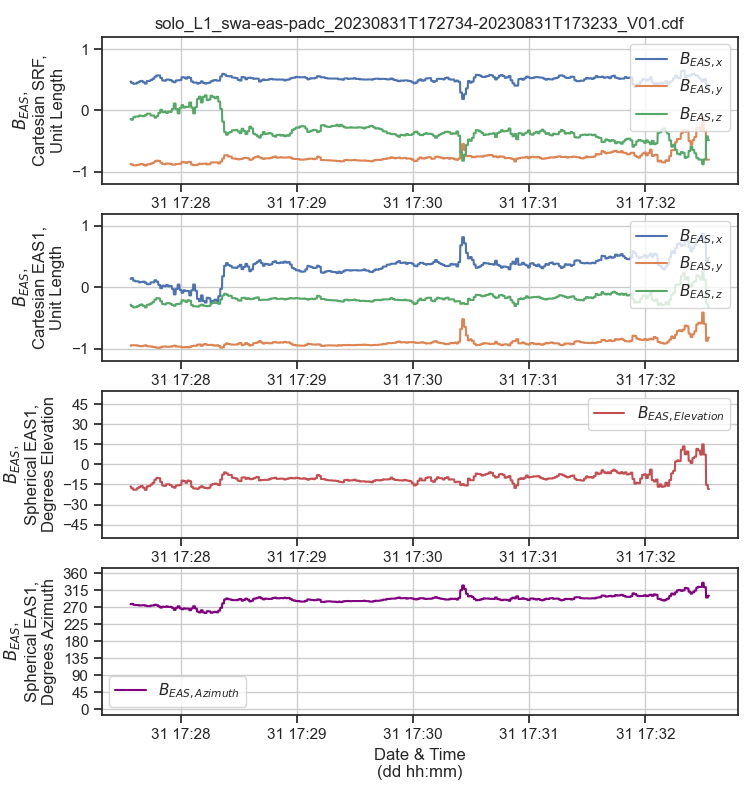
\includegraphics[width=1.05\linewidth]{figures/Transformation Example.png}
    \caption{Example \(B_{EAS}\) data from 31st August 2023. Top panel: Default cartesian \(B_{EAS}\) in SRF frame. 2nd panel: Cartesian \(B_{EAS}\) in EAS1 frame. 3rd panel: Elevation for spherical \(B_{EAS}\) in EAS1 frame. bottom panel: Azimuth for spherical \(B_{EAS}\) in EAS1 frame. The radius in spherical coordinates is not shown because all time series vectors are of length unity.}
    \caption*{Image Source: Author's own work}
    \label{fig: trans example}
\end{figure}

\(B_{EAS}\) and \(B_{MAG}\) are both acquired from SOAR in cartesian SRF coordinates. This is contrasted with data in cartesian radial-tangent-normal (RTN) coordinates (which are also provided for MAG\cite{soar}), where the \q{x-axis} is oriented radially away from the Sun, the \q{z-axis} is oriented towards the north celestial pole, and the \q{y-axis} is tangent to a prograde orbit in the plane of the ecliptic, completing the triad. SRF coordinates correspond to the \q{S/C Frame} shown in Figure \ref{fig: EAS schematic}, which is approximately equivalent to RTN coordinates with the \q{x and y} axes inverted. However, this equivalence depends on Solar Orbiter's pointing accuracy, meaning that transformations between rigidly-coupled onboard reference frames (e.g. SRF and the EAS Instrument frame in Figure \ref{fig: EAS schematic}) are generally expected to be more consistent than transformations between onboard reference frames and celestial reference frames such as RTN\cite{erofeev2019}.
\\

To determine the effect of \(B_{EAS}\) and \(B_{MAG}\) on EAS elevation/azimuth binning, these time series had to be converted from cartesian SRF coordinates to spherical EAS1/EAS2 coordinates in terms of radius and elevation and azimuth angles, where the head should be chosen such that \(B_{EAS}\) and/or \(B_{MAG}\) lie within that head's FOV. This was calculated in the following order: Cartesian SRF \(\rightarrow\) Cartesian EAS1/2 \(\rightarrow\) Spherical EAS1/2. This order was chosen because SOAR provides \q{EAS\textit{X}\_TO\_SRF} transformation matrices packaged with level 2 EAS data CDF files published under \q{solo\_L2\_swa-eas\textit{X}-nm3d-dnf\_\textit{YYYYMMdd}T\textit{hhmmss}-\textit{YYYYMMdd}T\textit{hhmmss}\_V01.cdf} where \textit{X} is the EAS head number (1 or 2). Despite being packaged with timestamped CDF files, these transformation matrices do not appear to change over time (nor should they be expected to change over time). The matrices can be trivially inverted to enable a Cartesian SRF \(\rightarrow\) Cartesian EAS1/2 transformation. The default and inverted forms are shown in Table \ref{tab: EASX to SRF}, as would be expected geometrically based on Figure \ref{fig: EAS schematic}.

\begin{table}[h!]
    \centering
    \(
    \begin{array}{cc}
        \text{EAS1 to SRF} & \text{SRF to EAS1} \\
        \begin{bmatrix}
        0 & -\frac{\sqrt{2}}{2} & +\frac{\sqrt{2}}{2}\\
        0 & +\frac{\sqrt{2}}{2} & +\frac{\sqrt{2}}{2}\\
        -1 & 0 & 0\\
        \end{bmatrix} &
        \begin{bmatrix}
        0 & 0 & -1\\
        -\frac{\sqrt{2}}{2} & +\frac{\sqrt{2}}{2} & 0\\
        +\frac{\sqrt{2}}{2} & +\frac{\sqrt{2}}{2} & 0\\
        \end{bmatrix}
        \\
        \\
        \text{EAS2 to SRF} & \text{SRF to EAS2} \\
        \begin{bmatrix}
        0 & -\frac{\sqrt{2}}{2} & +\frac{\sqrt{2}}{2}\\
        0 & -\frac{\sqrt{2}}{2} & -\frac{\sqrt{2}}{2}\\
        -1 & 0 & 0\\
        \end{bmatrix} &
        \begin{bmatrix}
        0 & 0 & -1\\
        -\frac{\sqrt{2}}{2} & -\frac{\sqrt{2}}{2} & 0\\
        +\frac{\sqrt{2}}{2} & -\frac{\sqrt{2}}{2} & 0\\
        \end{bmatrix}
        \\
        
    \end{array}
    \)\\
    \caption{A table of transformation matrices between SRF and EAS1/2 coordinates in cartesian space. The matrices in the left column were found on SOAR (in reality, \(\pm\sqrt{2}/2\) was approximated as \(\pm0.707\) on SOAR).} 
    \label{tab: EASX to SRF}
\end{table}

% in particular, the \textit{CartesianRepresentation(x,y,z)} object with the \textit{.represent()} method

Once in the EAS1/2 frame, the Cartesian EAS1/2 \(\rightarrow\) Spherical EAS1/2 transformation was calculated using the \textit{astropy} library for Python\cite{astropy2013}\cite{astropy2018}\cite{astropy2022}. Figure \ref{fig: trans example} shows an example of normalised \(B_{EAS}\) data from 31st August 2023 at each stage of transformation from unit cartesian SRF to unit spherical coordinates in the EAS1 frame. Since the \Beas\ vector time series is normalised from the start, a time series of the radius in spherical coordinates would be trivial and is not shown. In Figure \ref{fig: trans example}, the x-axis, y-axis, and z-axis in the top panel (cartesian SRF) appear to align most closely with the z-axis (+ an offset), the y-axis (+ an offset), and the opposite of the x-axis in the 2nd panel (cartesian EAS1) respectively. This is also expected based on the \q{S/C} and \q{EAS 1 Science} frames in Figure \ref{fig: EAS schematic}, further validating the matrices in Table \ref{tab: EASX to SRF}.
\\


\section{Preliminary \(B_{EAS}\)-\(B_{MAG}\) Comparison: Method}
As described in the author's earlier work, a preliminary comparison was performed between \(B_{EAS}\) and \(B_{MAG}\) from a small set of arbitrarily selected periods of Burst Mode data to justify the creation of a completeness score\cite{dickson2024}.
\\

\(B_{EAS}\) time series are stored in EAS burst mode CDF files under \q{EPOCH} for the time axis and \q{SWA\_EAS\_MagDataUsed} for the series axis. Similarly, \(B_{MAG}\) time series are stored in MAG SRF normal mode CDF files under \q{EPOCH} and \q{B\_SRF} respectively. Every \q{B\_SRF} vector was normalised before comparison with \(B_{EAS}\). The dot product between \(B_{EAS}\) and \(B_{MAG}\) vectors gives the angular offset between them. This angle was calculated for every vector in a few randomly chosen time series, yielding the results and discussion presented in Section \ref{prelim results}, confirming the risk of PAD incompleteness for a few example datasets to justify the eventual development of a completeness metric. 

\section{Simulating EAS Burst Mode Steering} \label{sim steering - method}

To better understand sources of error in Burst Mode data, the Burst Mode steering algorithm was simulated in Python using \(B_{EAS}\) vectors, Table \ref{fig: trans example}, and the latest published binning tables shown in Appendix \ref{appendixlabel1}. As per Section \ref{EAS Burst Mode}, the algorithm first requires a comparison between \(B_{EAS}\) and both EAS head aperture center planes in SRF coordinates, equivalent to their z-axes + 90\degree\ elevation in their respective EAS coordinates. This algorithm can be summarised as follows: 

\begin{enumerate}
    \item The angles between \(B_{EAS}\) and both EAS head aperture center planes are calculated.
    \item The smallest angle selects the EAS frame to which \(B_{EAS}\) is transformed, in spherical coordinates.
    \item The upper and lower bounds of the bin tables are compared to the elevation and azimuth angles of each vector in the spherical EAS frame until their correct bins are found.
\end{enumerate}

The anti-parallel vector to \(B_{EAS}\) is also determined and binned, resulting in two selected elevation bins. 
To validate the simulated binning algorithm, the time series for \(B_{EAS}\) can be plotted against the selected bin centers and upper and lower bounds. If head-selection has been performed correctly, then the \(B_{EAS}\) elevation component should never exceed \(\pm45\degree\). The results of this approach to validation were positive and are presented in Section \ref{sim steering}.
\\

The most direct way to validate the algorithm is to compare the simulated bins and heads selected to the actual bins and heads selected for a given dataset. EAS level 1 Burst Mode CDF data files on SOAR provide this information. The variable \q{SWA\_EAS\_EasUsed} contains a time series indicating the head selected (0 for EAS1, 1 for EAS2). \q{SWA\_EAS\_ElevationUsed} contains a 2D time series with the bin indices (0-15) of the elevation bins selected for parallel and anti-parallel \(B_{EAS}\). \q{SWA\_EAS\_ELEVATION}, \q{SWA\_EAS\_ELEVATION\_delta\_lower}, and \q{SWA\_EAS\_ELEVATION\_delta\_upper} contain 2D time series with the actual bin centers and boundaries used for the selected elevation bins (in degrees), for parallel and anti-parallel \(B_{EAS}\). In contrast, while there are similarly-named variables for azimuth (\q{SWA\_EAS\_AZIMUTH}, \q{SWA\_EAS\_AZIMUTH\_delta\_lower}, and \q{SWA\_EAS\_AZIMUTH\_delta\_upper}), these do not contain time series. Instead, the azimuth variables contain the constant bin center and delta data found in Table \ref{tab: Bin Table EAS Azimuth July 2021}. Therefore, simulated azimuth binning cannot be verified this way. This is of no consequence to Burst Mode simulation because steering is only determined by elevation binning.
\\

The results of this approach to validation led to the discovery of an error in the memory of the SWA Data Processing Unit (SWA-DPU). These results are also presented in Section \ref{sim steering}.

\section{Visualisation for Bins and Vectors} \label{visualisation}
To facilitate the determination of Burst Mode data accuracy, a visualisation tool was developed for this project based on a plot produced by Owen et al (2021)\cite{owen2021}. This was the tool that was used to create Figures \ref{fig: all bins}, \ref{fig: normal - full contours}, and \ref{fig: normal - full contours + selection} in Section \ref{EAS PAD}. This visualisation is attractive because it concisely displays magnetic field vectors in SRF, circumventing the need to change coordinates following a sensor head change. The choice of SRF over RTN has been justified in Section \ref{coordinate systems}. This approach to visualisation also allows the difference in angular bin widths to be seen projected on to the sky, visualising each head and pixel's field of view along with \Beas\ vectors in a form that may facilitate a more intuitive determination of the ensuing effects on Burst Mode steering compared to other approaches.
\\

The visualisation was implemented in Python. The first step was to plot the grid of angular EAS bins in SRF space. Plotting the grid is easily (though inefficiently) accomplished in the EAS1/2 frame using spherical coordinates by simply plotting many closely-spaced points in straight lines along the upper and lower bounds of the elevation and azimuth bin tables (see Appendix \ref{appendixlabel1}). This step is described in detail with added excerpts of code from its implementation in Appendix \ref{appendixlabel2}. Plotting the parallel and anti-parallel magnetic field vectors seen in Figures \ref{fig: normal - full contours} and \ref{fig: normal - full contours + selection} was also relatively straightforward. Since both \(B_{EAS}\) and \(B_{MAG}\) are acquired from SOAR in SRF coordinates, they only had to be transformed to spherical coordinates and plotted with distinct markers to differentiate them. The markers used throughout this report are a diamond for the parallel vector and a square for the anti-parallel vector. \(B_{EAS}\) and \(B_{MAG}\) vectors are also differentiated by colour (green and purple respectively).
\\

To plot the contours of constant pitch angle at arbitrary pitch angles around these vectors involved adapting an algorithm written by Dr. Chris Owen in Interactive Data Language (IDL). The algorithm starts by constructing the transformation matrix \textit{M} from a cartesian reference frame whose z-axis is aligned with the magnetic field vector to cartesian SRF coordinates. \textit{M} is constructed using the elevation and azimuth for a magnetic field vector \(B\) in spherical SRF coordinates as per Equation \ref{eq: Matrix M}, where \(\theta=\textrm{(spherical SRF magnetic field elevation)}*\pi/180\degree\) and \(\phi=\textrm{(spherical SRF magnetic field azimuth)}*\pi/180\degree\).

\begin{equation} \label{eq: Matrix M}
    M=
    \begin{bmatrix}
    \cos{\phi}\cos{\theta} & -\sin{\phi} & -\cos{\phi}\sin{\theta}\\
    \sin{\phi}\cos{\theta} & \cos{\phi} & -\sin{\phi}\sin{\theta}\\
    \sin{\theta} & 0 & \cos{\theta}\\
    \end{bmatrix}
\end{equation}

From there, the proceeding algorithm can be summarised as follows:
\begin{enumerate}
    \item For a given contour with pitch angle \(\alpha\), calculate the angular length (conceptually similar to \q{circumference}) of the contour in spherical SRF coordinates. Multiply this by the angular point density to yield a number of phase angles \(\varphi\) around \(B\) with which to plot points along the contour. \(\varphi\) is analogous to azimuth in the \(B\)-aligned frame.
    \item Working in the \(B\)-aligned frame, for every phase angle \(\varphi\), construct the cartesian vector \(\vec{p}_B\) according to:
    \begin{equation} \label{eq: contour vector construction}
        \centerfloat
        \vec{p}_B=
        \begin{bmatrix}
        x_{\alpha,\varphi}\\
        y_{\alpha,\varphi}\\
        z_{\alpha,\varphi}\\
        \end{bmatrix}
        =
        \begin{bmatrix}
        \cos{\alpha}\\
        \sin{\alpha}\cos{\varphi}\\
        \sin{\alpha}\sin{\varphi}\\
        \end{bmatrix}
    \end{equation}
    \item Transform \(\vec{p}_B\) into \(\vec{p}_{SRF}\) in the cartesian SRF frame using \textit{M} according to:
    \begin{equation} \label{eq: contour vector transform}
        \vec{p}_{SRF}=M\vec{p}_B
    \end{equation}
    \item Transform \(\vec{p}_{SRF}\) to spherical SRF coordinates, and its elevation and azimuth angles can be plotted directly.
\end{enumerate}
\\

Following this algorithm to plot all vectors for all phase angles in the range \([0\degree,360\degree]\) with appropriate increments and all pitch angles in the range \([0\degree,180\degree]\) in 15\degree\ increments yields Figure \ref{fig: normal - full contours} when plotted alongside EAS bins and the \Beas\ vector itself for the appropriate date and time.
\\

\begin{figure}[h!]
    \centering
    \centerfloat
    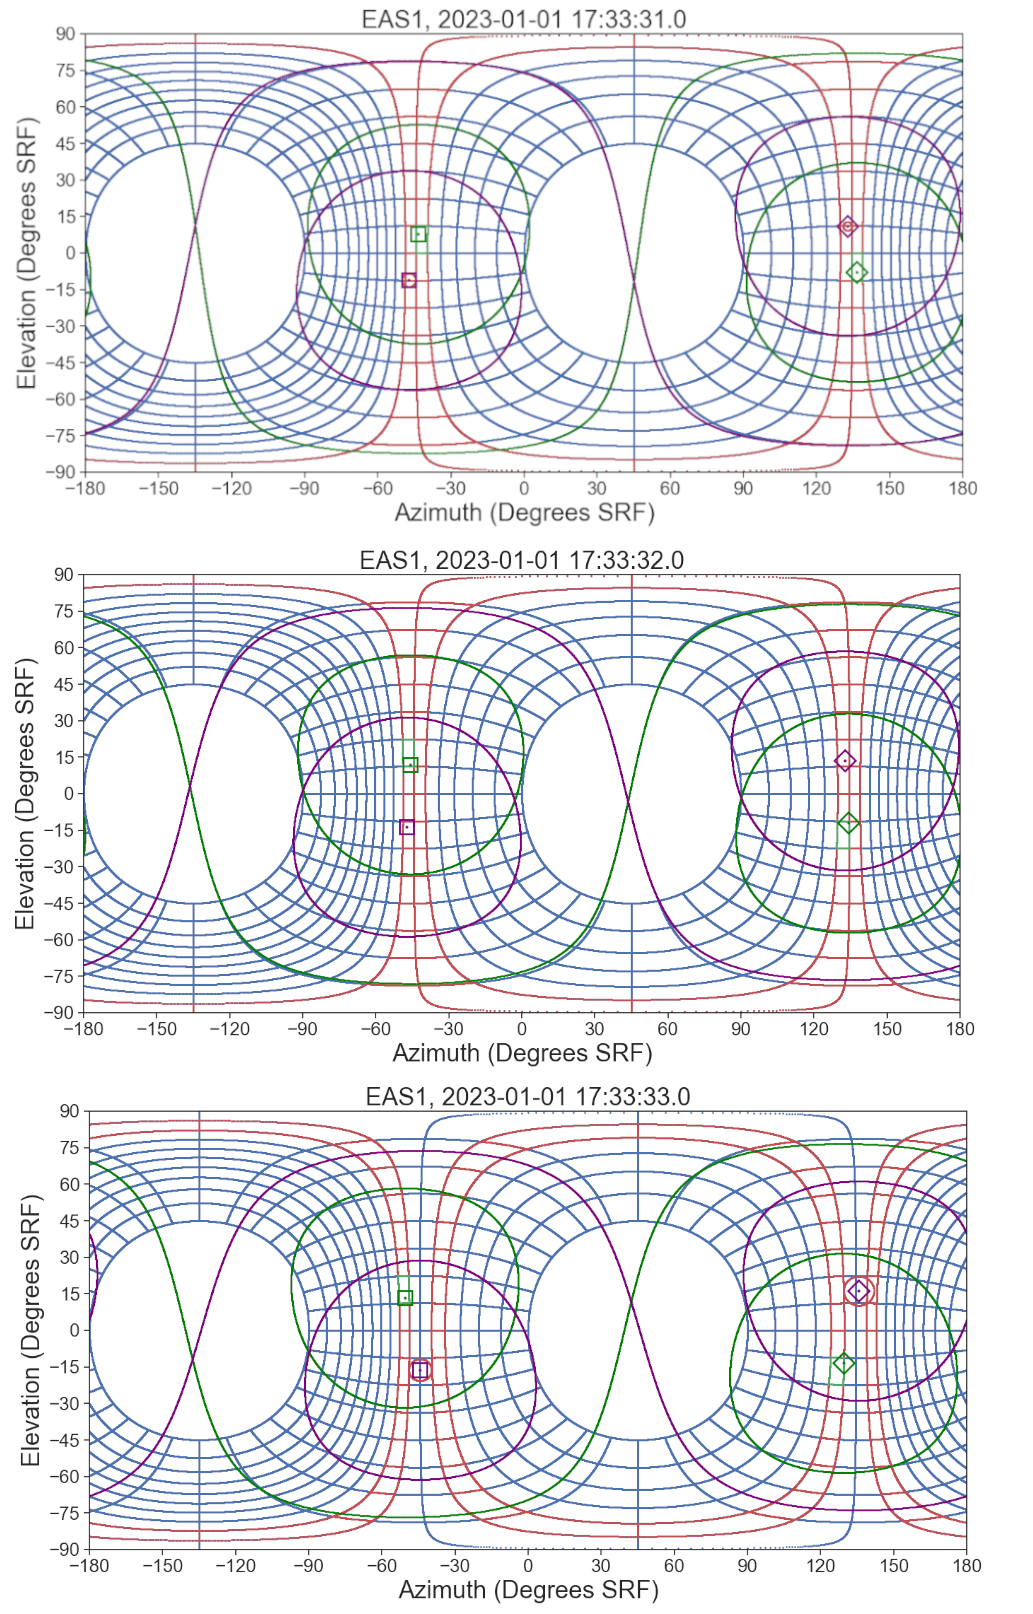
\includegraphics[width=0.84\linewidth]{figures/anim_example.png}
    \caption{Three frames of an animation produced by plotting \Beas\ and \Bmag\ data from 1st January 2023 along with pitch angle contours including loss contours, which are described in Section \ref{completeness}. Green represents \Beas\ and purple represents \Bmag. Diamond and square markers represent parallel and anti-parallel magnetic field vectors respectively. Top panel: Data from 17:33:31 UTC. Middle panel: Data from 17:33:32 UTC. Bottom panel: Data from 17:33:33 UTC.}
    \caption*{Image Source: Author's own work}
    \label{fig: animation example}
\end{figure}
\\
\newpage

As SOAR's magnetic field vector data comes in time series, this tool can also be used to visualise magnetic field variation over time in the form of an animation. Individual frames of an animation can be generated for every data point in a magnetic field time series, and then combined into a high-definition \textit{.gif} using the \textit{imageio} library for Python\cite{klein2024_imageio}\footnote{Other methods for composing \textit{.gif} files are available and may be more straightforward. One of the most straightforward methods is to use free online \q{image-to-gif} converters, but the resolution of \textit{.gif} files acquired by this method was found to be too low for this project's purposes.}. To play the animation at a realistic frame rate, the duration of each frame must be specified. For Burst Mode data, the duration is set to 0.125s, matching the time delay between successive time series vectors. Using data from 1st January 2023, three (non-consecutive) frames of such an animation, 1s apart, are included in Figure \ref{fig: animation example} for example.
\\

\section{S20 Link Latency} \label{S20 method}
It is possible that some of the \(B_{EAS}\)-\(B_{MAG}\) discrepancy can be attributed to latency over the S20 inter-instrument data link\cite{owen2021}.  This latency may be particularly noticeable on 1/8th second timeframe during periods of heavy data traffic\cite{owen2021}. If noticeable, then the latency is expected to cause a time delay between \(B_{EAS}\) and \(B_{MAG}\) where \(B_{MAG}\) leads by at least \(\sim\)0.125s. One approach to measuring this time delay is to perform a cross-correlation analysis between \(B_{EAS}\) and \(B_{MAG}\)\cite{hanus2019}); in principle, a cross-correlation function (CCF) takes a domain of time delays as input and the delay that gives the strongest correlation between the two time series can be selected to represent the latency. The principle behind this approach is well-illustrated by Figure \ref{fig: Hanus CCF} by Hanus et al\cite{hanus2019} for two 1D time series \(x(t)\) and \(z(t)\) and latency \(\tau_0\).
\\

\begin{figure}[h!]
    \centering
    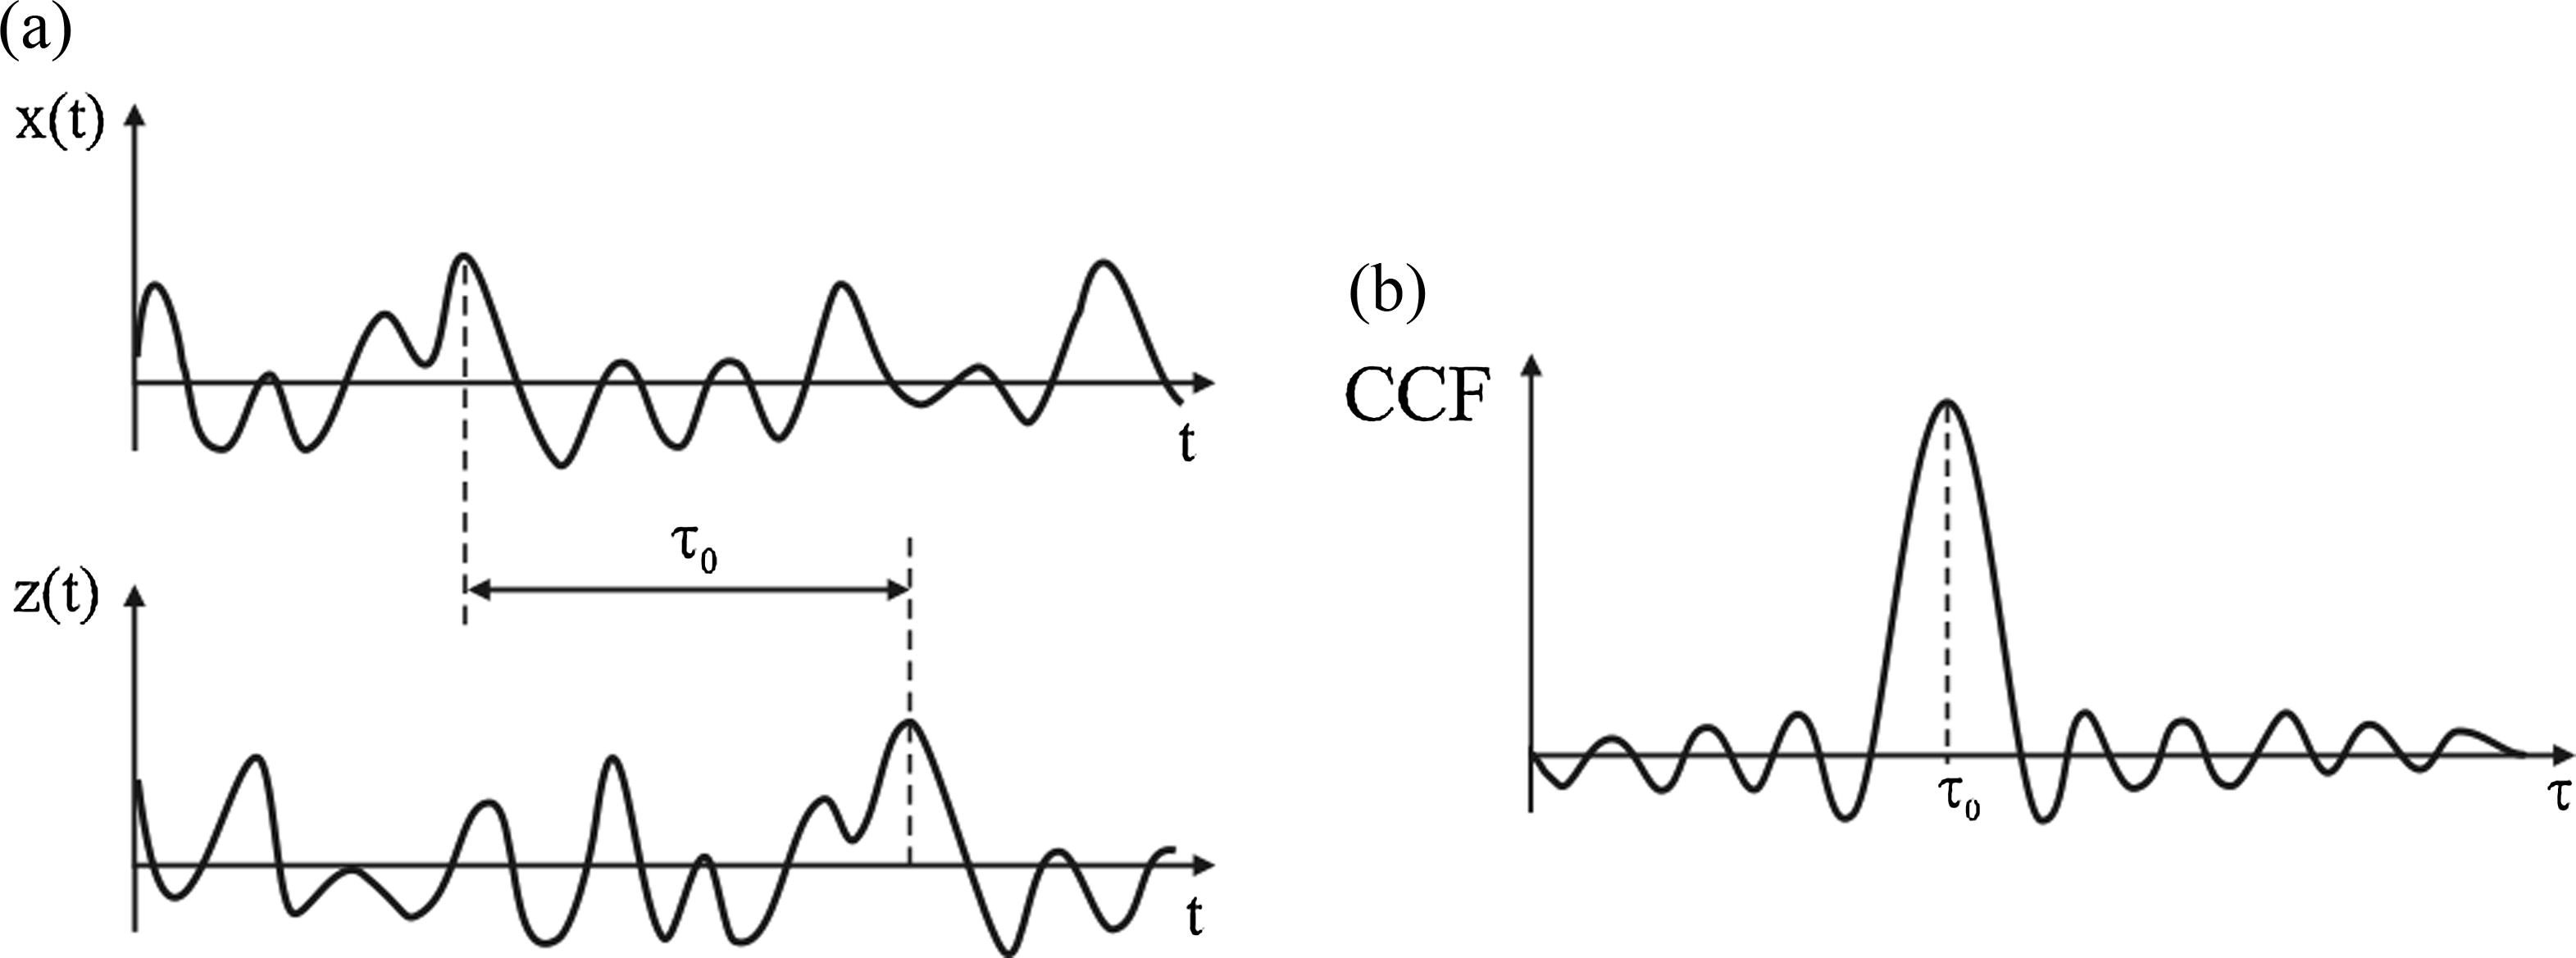
\includegraphics[width=1\linewidth]{figures/hanus diagram.jpg}
    \caption{Two figures illustrating CCF time delay determination. (a): Two arbitrary time series \(x(t)\) and \(z(t)\), which are well-approximated as identical time series with a time delay \(\tau_0\) between them. (b): A plot of the CCF applied to \(x(t)\) and \(z(t)\), showing maximum correlation at the time delay \(\tau_0\), representing the latency.}
    \caption*{Image Source: Hanus et al\cite{hanus2019}}
    \label{fig: Hanus CCF}
\end{figure}

A version of the cross-correlation approach was implemented in Python to calculate the S20 latency \(\tau_{S20}\). The \textit{scipy} library for Python provides a wide range of signal processing methods and functions, including CCFs\cite{2020SciPy}. Given two 1D arrays of data, the discrete CCF between them can be determined using the \textit{scipy.signal.correlate()} method\cite{2020SciPy}. The discrete CCF generated by this method is an approximation of a theoretical CCF between two complex, 1D functions \(f(t)\) and \(g(t)\) over time \textit{t}. The CCF, sometimes denoted \q{\(f\star g\)}, is generated by convolving \(g(t)\) with the complex conjugate of \(f(t)\), \(\overline{f}(t)\) according to:

\begin{equation} \label{eq: continuous CCF}
    f\star g=\overline{f}(-t)\ast g(t)
\end{equation}

where convolution is denoted by \q{\(\ast\)}\cite{bracewell1986}\cite{CCFs}. Convolution is defined by:

\begin{equation} \label{eq: convolution}
    (f\ast g)(t)=\int_{-\infty}^{\infty}f(\tau)g(t-\tau)d\tau
\end{equation}

where \(\tau\) denotes the continuously-variable displacement in time between \(f(t)\) and \(g(t)\)\cite{CCFs}, also known as the \textit{lag}. Combining Equations \ref{eq: continuous CCF} and \ref{eq: convolution} and changing integration variables from \textit{t} to \(\tau\) yields Equation \ref{eq: continuous CCF integral} for the cross-correlation in terms of \(\tau\):

\begin{equation} \label{eq: continuous CCF integral}
    (f\star g)(\tau)=\int_{-\infty}^{\infty}\overline{f}(t)g(t+\tau)dt
\end{equation}

Equation \ref{eq: continuous CCF integral} can be expressed in its discrete form in terms of discrete functions \(f(t)\) and \(g(t)\), yielding:

\begin{equation} \label{eq: discrete CCF}
    \textrm{CCF}\equiv(f\star g)(\tau)=\sum_{-\infty}^{\infty}\overline{f}(t)g(t+\tau)
\end{equation}

This is the definition of \q{CCF} that will be used for the remainder of this section\cite{2020SciPy}\cite{rabiner1978}. The translation of Equation \ref{eq: discrete CCF} into Python is given by \textit{scipy.signal.correlate()}. The array of lags \(\tau\) is generated by \textit{scipy.signal.correlation\_lags()}, which depends on the sample rate of \(f(t)\) and \(g(t)\) to define the timescale of \(\tau\). For this project, that is equivalent to the EAS Burst Mode sample rate of 8Hz. With the CCF and the array of lags, the latency \(\tau_0\) can be estimated by calculating the maximum of the CCF and finding its corresponding lag.
\\

\begin{figure}[h!]
    \centering
    \centerfloat
    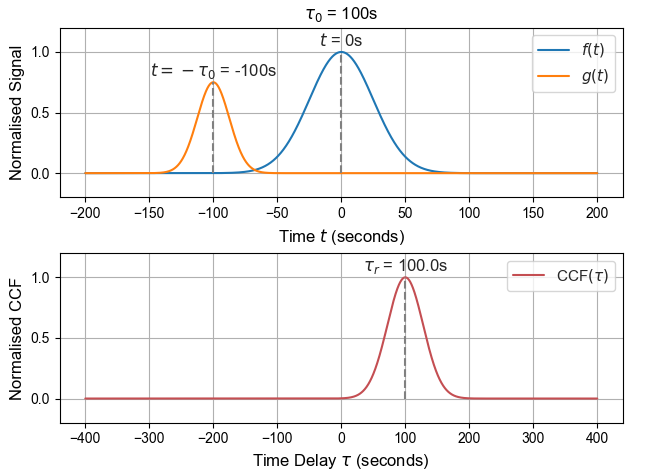
\includegraphics[width=1\linewidth]{figures/Time Delay Tests - Clean.png}
    \caption{Two figures illustrating the time delay algorithm for dummy data. Top panel: Normalised dummy time signals \(f(t)\) and \(g(t)\) plotted over 400s with a time delay \(\tau_0\) between them. The peaks of \(f(t)\) and \(g(t)\) are labelled with their time values. Bottom panel: The CCF of \(f(t)\) and \(g(t)\) plotted over 800s of time delays \(\tau\). The peak of the CCF is labelled with its value for the time delay \(\tau_r\approx \tau_0\).}
    \caption*{Image Source: Author's own work}
    \label{fig: time delay tests - clean}
\end{figure}

This time delay algorithm was implemented and validated using dummy time series data consisting of two Gaussian signals, \(f(t)\) and \(g(t)\) as shown in the upper half of Figure \ref{fig: time delay tests - clean}. \(f(t)\) has amplitude \(a_f=1\) and standard deviation \(\sigma_f=25\)s, and \(g(t)\) has \(a_g=0.75\) and \(\sigma_g=12.5\)s. \(f(t)\) and \(g(t)\) are distributed over 400s with \(N=3200\) data points to simulate the Burst Mode sample rate of 8Hz. There is a delay \(\tau_0=100\)s between \(f(t)\) and \(g(t)\), with \(f(t)\) in the lead. In the lower half of Figure \ref{fig: time delay tests - clean}, the calculated and normalised CCF is plotted against the array of lags over twice the duration of \(f(t)\) and \(g(t)\), showing a clear Gaussian peak at the value of \(\tau_0\) that it recovered from the comparison of \(f(t)\) and \(g(t)\), which is denoted \(\tau_r\). Figure \ref{fig: time delay tests - clean} shows reassuring results, correctly recovering a value of \(\tau_r=100.000\textrm{s}=\tau_0\). 
\\

The issue now is to determine the uncertainty in the calculated value. There is not much consensus on the \q{correct} approach to measuring the uncertainty CCF lags\cite{peterson1998}\cite{efron1992}. Peterson et al (1998) suggest Monte Carlo simulations of many small variations on the same cross-correlation to evaluate the sensitivity of the lag solution to individual data points. Specifically, they suggest a statistical test where the time series subject to the CCF is reduced to a large number of randomly selected subsets of the original dataset, each of which is shrunken by a factor \(\sim 1/e \approx0.37\). These subsets are each subjected to the CCF in the same way as before, allowing the calculation of a mean and standard deviation which provide a conservative estimate of the uncertainty. The principle behind this method inspired the implementation of a Python algorithm for calculating the uncertainty on the lag. The algorithm can be summarised as follows for arrays to be correlated, \(f\) and \(g\):
\begin{enumerate}
    \item Define two empty arrays \(f_i\) and \(g_i\). These will be the subset arrays.
    \item Starting from 0, take a random integer \q{step} through the indices of the arrays \(f\) and \(g\) and select their corresponding values to append to \(f_i\) and \(g_i\) respectively. The average length of the step should be \(\approx e\) to get the \(\sim1/e\) shrink factor (e.g. the first values might be randomly distributed around \(f(3)\) and \(g(3)\)).
    \item Repeat step 2 until the end of \(f\) and \(g\) is reached, and then cross-correlate \(f_i\) and \(g_i\) to calculate \(\tau_r\), dividing the sample rate by the average step length to reflect the subset's new data rate.
    \item Repeat steps 1 through 3 over \textit{M} iterations, and calculate the mean time delay \(\tau_r\) and standard deviation \(\sigma\) of the resulting collection of \(\tau_r\) values. \(\sigma\) is said to represent the uncertainty in \(\tau_r\).
\end{enumerate}
\\

\begin{figure}[h!]
    \centering
    \centerfloat
    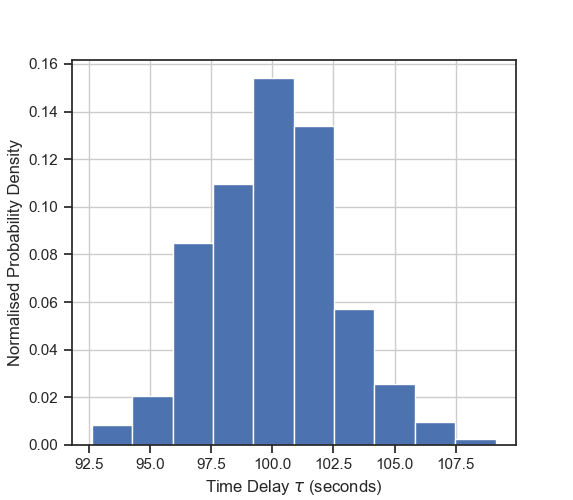
\includegraphics[width=0.8\linewidth]{figures/dummy hist.png}
    \caption{A histogram of the probability density function describing the \(M=1000\) simulations used to calculate the uncertainty in \(\tau_r\) for the dummy data used in Figure \ref{fig: time delay tests - clean}. There are 10 equally-spaced time delay bins.}
    \caption*{Image Source: Author's own work}
    \label{fig: dummy hist}
\end{figure}

\noindent The algorithm was validated using the same dummy data shown in Figure \ref{fig: time delay tests - clean}. In this case, the average step length was set to 3, and the random steps were calculated using a uniform random variable in the inclusive range \((1,5)\). After \(M=1000\) iterations, a value of \(\tau_r=100.0\textrm{s}\pm2.6\textrm{s}\) was acquired. A probability density histogram resulting from the Monte Carlo simulation is shown in Figure \ref{fig: dummy hist}. While an uncertainty of \(\pm2.6\textrm{s}\) is too small to be displayed on a plot of the same scale as Figure \ref{fig: time delay tests - clean}, it is significantly larger than the time resolution of 8Hz magnetic field data. Given that the dummy data used in this exercise are, by design, much \q{cleaner} than real magnetic field time series, this suggests a restrictive lower bound on the resolution of S20 data link latency determination using this method. The results of further experiments using real magnetic field data are presented in Section \ref{S20 Link Latency}.

% Further validation tests were performed by adding Gaussian noise to \(f(t)\) and \(g(t)\) with an arbitrary scale \(\sigma_n=0.05\). This was meant to evaluate the algorithm's performance in response to more realistic, non-uniform signals. An example of these tests is shown in Figure \ref{fig: time delay tests - noisy}. 10,000 of these tests were performed, yielding a mean \(\langle\tau_r\rangle=99.965\)s with standard deviation \(\sigma=0.547\)s.

% \begin{figure}[h!]
%     \centering
%     \centerfloat
%     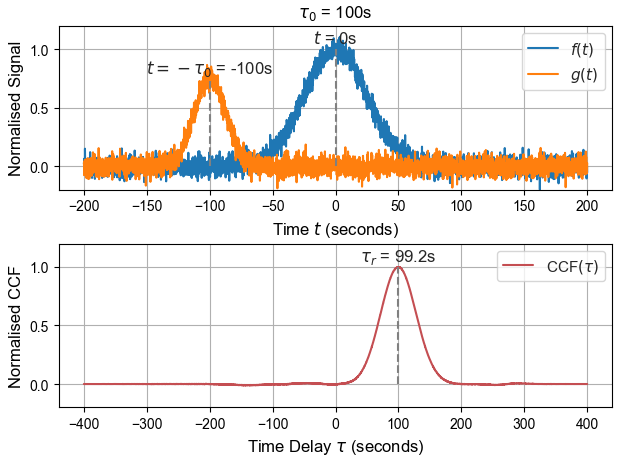
\includegraphics[width=1\linewidth]{figures/Time Delay Tests - Noisy.png}
%     \caption{Two more figures illustrating the time delay algorithm for the dummy data shown in Figure \ref{fig: time delay tests - clean} with added Gaussian noise. Top panel: \(f(t)\) and \(g(t)\) + Gaussian noise of scale \(\sigma_n=0.05\). Peaks labelled with time values. Bottom panel: The CCF of \(f(t)\) and \(g(t)\) + noise, peak labelled with \(\tau_r\).}
%     \caption*{Image Source: Author's own work}
%     \label{fig: time delay tests - noisy}
% \end{figure}

% Having been validated on dummy data, the next step is to apply this lag algorithm to real magnetic field time series.

\chapter{Results and Discussion}
\label{chapterlabel3}

\section{Preliminary \Beas-\Bmag\ Comparison: Results} \label{prelim results}
The angle between \Beas\ and \Bmag\ vectors, when plotted alongside those vectors for randomly chosen sample data from 31st August 2023, yields Figure \ref{fig: angle example august}.
\\

\begin{figure}[h!]
    \centering
    \centerfloat
    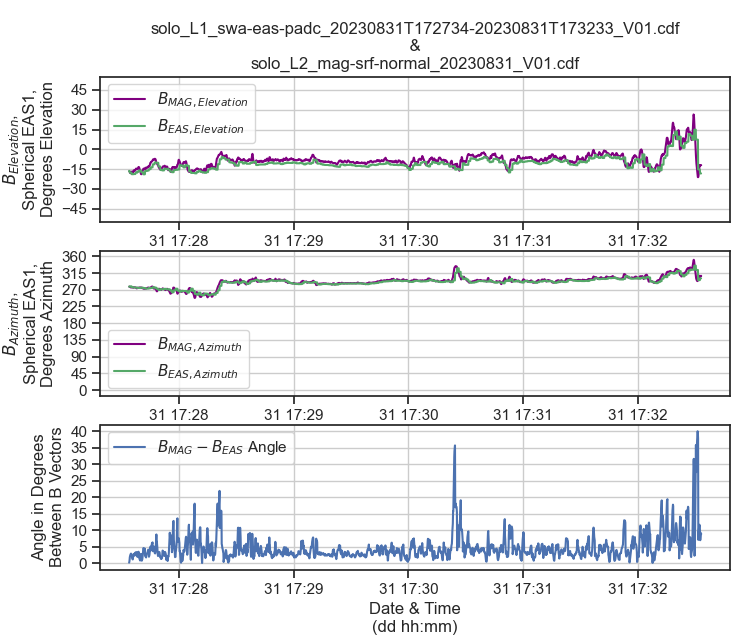
\includegraphics[width=1.05\linewidth]{figures/Angle Example.png}
    \caption{Example \(B_{EAS}\) data from a 5 minute period of EAS Burst Mode on 31st August 2023. Top panel: Elevation for \(B_{EAS}\) and \(B_{MAG}\) in spherical EAS1. Middle panel: Azimuth for \(B_{EAS}\) and \(B_{MAG}\) in spherical EAS1. Bottom panel: Angular difference between \(B_{EAS}\) and \(B_{MAG}\).}
    \caption*{Image Source: Author's own work}
    \label{fig: angle example august}
\end{figure}

\begin{figure}[h!]
    \centering
    \centerfloat
    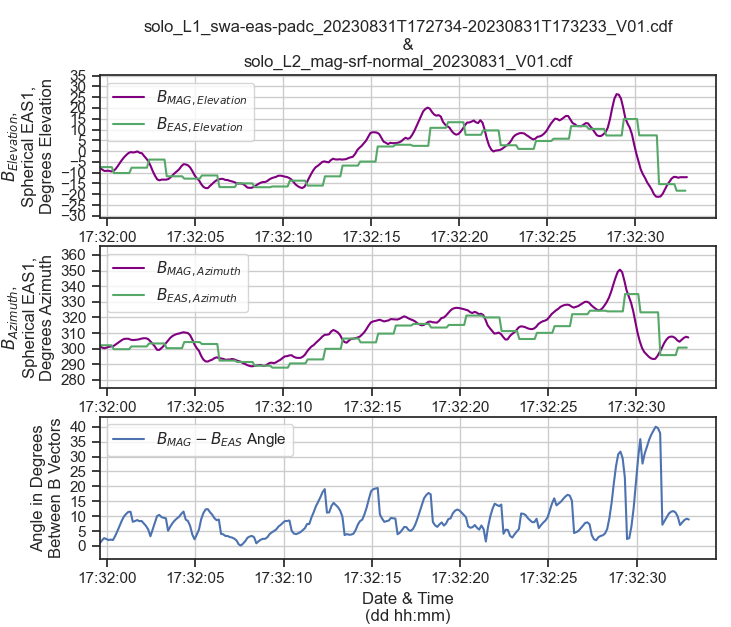
\includegraphics[width=1.05\linewidth]{figures/Angle Example Detail.png}
    \caption{A detailed look at the last \(\sim5\)s of Figure \ref{fig: angle example august}. Top panel: Elevation for \(B_{EAS}\) and \(B_{MAG}\) in spherical EAS1. Middle panel: Azimuth for \(B_{EAS}\) and \(B_{MAG}\) in spherical EAS1. Bottom panel: Angular difference between \(B_{EAS}\) and \(B_{MAG}\).}
    \caption*{Image Source: Author's own work}
    \label{fig: angle example detail august}
\end{figure}

By inspection, while relatively good agreement can be seen between \(B_{EAS}\) and \(B_{MAG}\) over long timescales, there are clear discrepancies over short timescales as shown in Figure \ref{fig: angle example detail august}. An unexpected observation is that \(B_{EAS}\) has less time resolution than \(B_{MAG}\), appearing only to update at 1Hz. Inspection of the raw \q{SWA\_EAS\_MagDataUsed} data time series data reveals that while this data array \textit{is} published to SOAR with 8 vectors for every second of \q{EPOCH} as advertised, these vectors are only updated once per second, resulting in 8 identical vectors per second such that the effective cadence is 1Hz. Since these data are packaged in L1 \textit{.cdf} files, they are expected to represent the true MAG data used to steer EAS, which implies that the alleged 1/8th second resolution of EAS Burst Mode is compromised by a magnetic field vector only updates at 1Hz. This will be a particular source of error during periods of fast-changing magnetic field. This effective 1Hz effect has been observed in other periods of Burst Mode from the sample including 5th November 2023 and 1st January 2023. It is absent from the relatively quiet period on 30th May 2023. Further research is required to determine the cause for this unexpectedly low update cadence, and how widespread of an issue this is in the SOAR dataset.
\\

The highest angular offset in Figure \ref{fig: angle example august} is observed to exceed 40\(\degree\), and it exceeds 70\(\degree\) in a different example from 5th November 2023. Otherwise, the offset is between \(0\degree\) and \(10\degree\) for \(\sim82\%\) of the period in Figure \ref{fig: angle example august}. In comparison, the offset varies between \(3\degree\) and \(5\degree\) for \(\sim80\%\) of the period in a different example from 30th May 2023, and between \(6\degree\) and \(8\degree\) for the remaining period. The bin centers and bin widths for elevation and azimuth are tabulated with level 2 EAS data files. While azimuth bins are identical for both heads, elevation bins are different due to minor differences in the assembly of each EAS head's electron optics. These tables have been updated over time but remained constant from 17th July 2021 until January 2024, when they were reverted to a previous version due to the error described in Section \ref{sim steering}. The tables from that 2021-2024 period are discussed here and are included in Appendix \ref{appendixlabel1}. The widest angular bin in EAS1 has width \(\pm6.06\degree\). This is well below much of the angular offset observed in the sample, therefore, it is established that \Beas\ could be sufficiently offset from \Bmag\ to cause erroneous Burst Mode steering, justifying the development of a metric for PAD quality/completeness.
\newpage

\section{SWA-DPU Binning Algorithm} \label{sim steering}

\begin{figure}[h!]
    \centering
    \centerfloat
    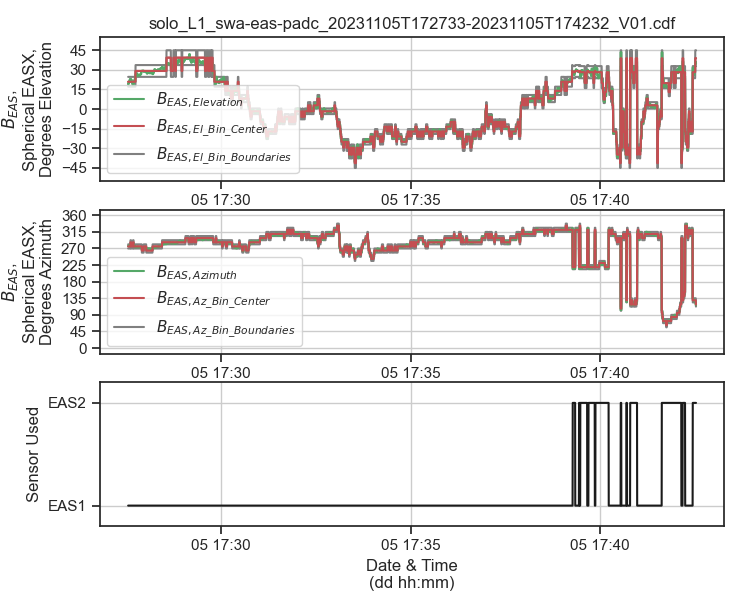
\includegraphics[width=1.05\linewidth]{figures/Steering Example.png}
    \caption{Example \(B_{EAS}\) data from a 15-minute period of EAS Burst Mode on 5th November 2023 showing a simulation of the Burst Mode steering algorithm. The reference frame for the top two panels is labelled \q{EASX} to indicate that it switches between EAS1 and EAS2 over the 15 minute period depending on \(B_{EAS}\) orientation and resulting head selection. Top panel: Elevation for \(B_{EAS}\) in spherical EASX coordinates, along with the centers and upper/lower bounds of the selected elevation bins (\q{El\_Bin\_Center} and \q{El\_Bin\_Boundaries} respectively). Middle panel: Azimuth for \(B_{EAS}\) in spherical EASX coordinates, along with the centers and upper/lower bounds of the selected azimuth bins (\q{Az\_Bin\_Center} and \q{Az\_Bin\_Boundaries} respectively). Bottom panel: The selected head over time.}
    \caption*{Image Source: Author's own work}
    \label{fig: steering example november}
\end{figure}

In the interest of validating the simulated binning algorithm described in Section \ref{sim steering - method}, the simulated binning for parallel \Beas\ vectors is plotted in Figures \ref{fig: steering example november} and \ref{fig: steering example november detail} along with a plot of the chosen head over time, for a 15-minute period on 5th November 2023. Figure \ref{fig: steering example november} shows that the elevation and azimuth values \q{jump} as the reference frame switches from EAS1 to EAS2 towards the end of the time series. As expected, this switch can be triggered by the \(B_{EAS}\) elevation exceeding \(\pm45\degree\) in its previous head's reference frame. Figure \ref{fig: steering example november detail} provides a detailed view of the algorithm's selection of appropriate binning such that the \(B_{EAS}\) trace stays between bin boundaries.
\\

\begin{figure}[h!]
    \centering
    \centerfloat
    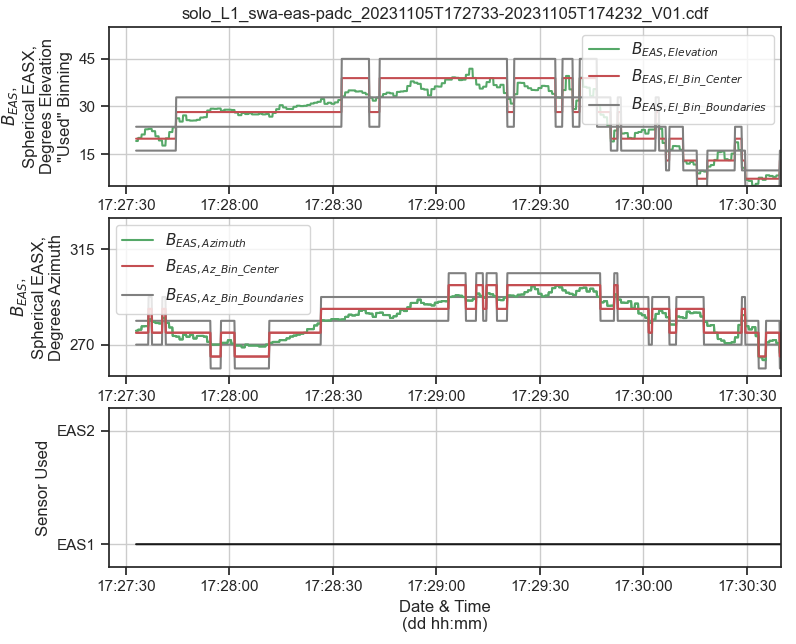
\includegraphics[width=1.05\linewidth]{figures/Steering Example Detail Start.png}
    \caption{A detailed view of the first \(\sim2.5\) minutes of Figure \ref{fig: steering example november}. Top panel: Elevation + binning for \(B_{EAS}\) in spherical EASX coordinates. Middle panel: Azimuth + binning for \(B_{EAS}\) in spherical EASX coordinates. Bottom panel: The selected head over time.}
    \caption*{Image Source: Author's own work}
    \label{fig: steering example november detail}
\end{figure}

In the interest of validating the binning algorithm even further, a more direct comparison was performed using the \q{Used} bin data directly from SOAR \textit{.cdf} files. Plotting the \q{Used} heads and elevation bins in an attempt to recreate Figure \ref{fig: steering example november} yields Figure \ref{fig: november bin error}. While the \q{SWA\_EAS\_EasUsed} head is perfectly correlated with the calculated head in the bottom panel of Figure \ref{fig: november bin error}, the top panel shows that not only does the \q{SWA\_EAS\_ELEVATION} binning appear to disagree with the simulated binning in the top panel of Figure \ref{fig: november bin error}, but the \q{Used} binning also appears to capture the \Beas\ elevation inaccurately over long periods of the time series. This is shown more clearly in Figure \ref{fig: november bin error detail}. In an attempt to fix this discrepancy, the data binning code was reviewed and multiple variations of the elevation bin tables were applied to the simulated algorithm. A possible bug was considered that might have caused the bin tables for the two heads to be swapped, but swapping them manually did not fix the discrepancy. The possibility that the uploaded data on SOAR had been reverted to a previous version was also considered, and older bin tables available on SOAR from 19th August 2020 to 17th July 2021, and from Solar Orbiter's commissioning to 19th August 2020 were also applied, but these did not fix the discrepancy either. The discrepancy was brought to the attention of the Principal Investigator of Solar Orbiter SWA (Dr. Chris Owen) and the SWA operations team, and Solar Orbiter was commanded to downlink the binning tables in its memory along with routine housekeeping data. The data downlink revealed that Solar Orbiter had, indeed, been using outdated bin tables in the SWA-DPU onboard, explaining the failure of \q{SWA\_EAS\_ELEVATION\_delta\_lower} and \q{SWA\_EAS\_ELEVATION\_delta\_upper} to encapsulate \Beas. 
\\

\begin{figure}[h!]
    \centering
    \centerfloat
    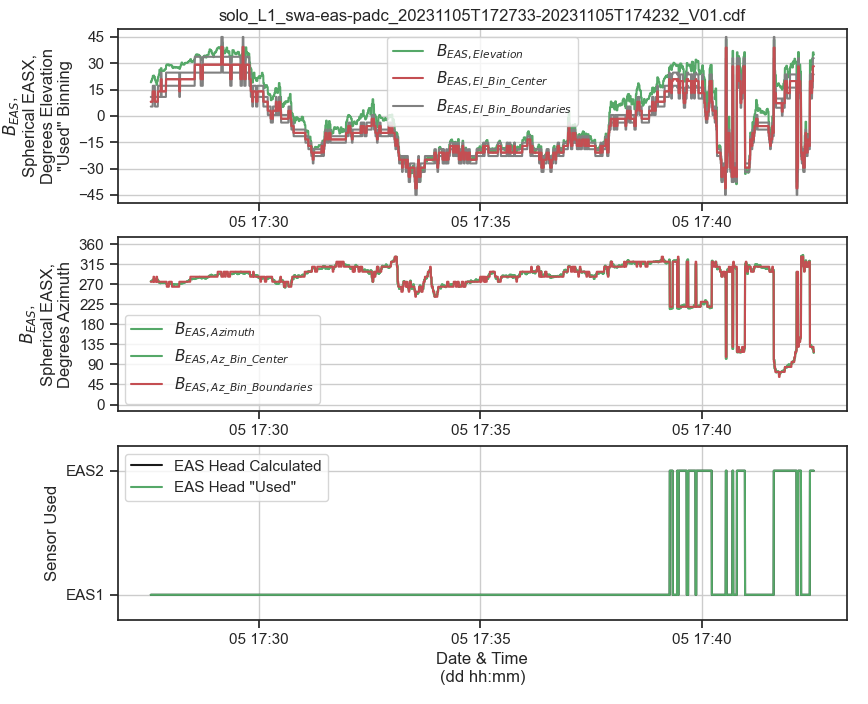
\includegraphics[width=1.05\linewidth]{figures/Steering Example (bin issue).png}
    \caption{Similar data to Figure \ref{fig: steering example november}, but plotting the \q{Used} bin centers, bin bounds, and sensor heads. Top panel: Elevation for \(B_{EAS}\) in spherical EASX coordinates, along with centers and upper/lower bounds of the used elevation bins (\q{El\_Bin\_Center} and \q{El\_Bin\_Boundaries} respectively). Middle panel: Azimuth for \(B_{EAS}\) in spherical EASX coordinates, along with the centers and upper/lower bounds of selected azimuth bins (\q{Az\_Bin\_Center} and \q{Az\_Bin\_Boundaries} respectively). Bottom panel: The selected, or \q{Calculated} head and used head over time.}
    \caption*{Image Source: Author's own work}
    \label{fig: november bin error}
\end{figure}

\begin{figure}[h!]
    \centering
    \centerfloat
    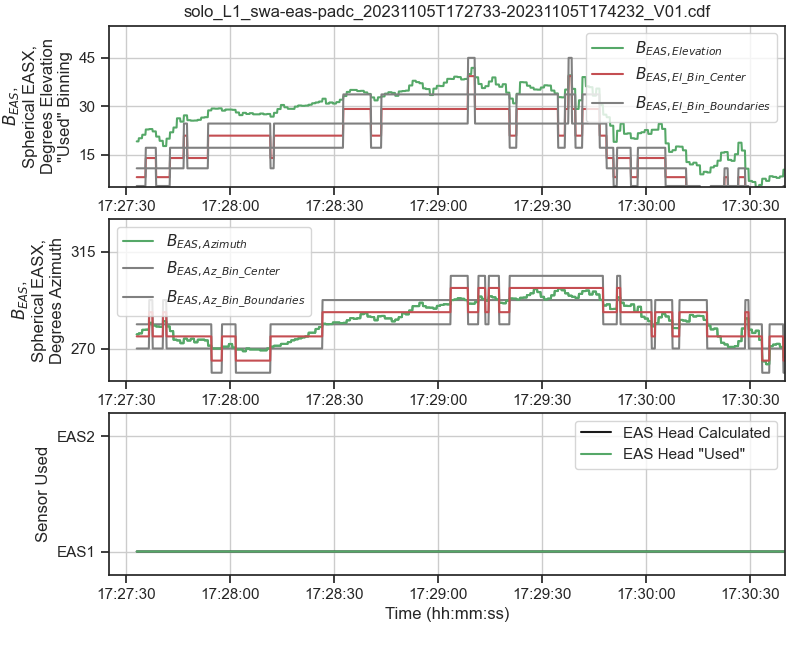
\includegraphics[width=1.05\linewidth]{figures/Steering Example Detail Start (bin issue).png}
    \caption{A detailed view of the first \(\sim2.5\) minutes of Figure \ref{fig: steering example november}. Top panel: Elevation + used binning for \(B_{EAS}\) in spherical EASX. Middle panel: Azimuth + binning for \(B_{EAS}\) in spherical EASX. Bottom panel: The selected, or \q{Calculated} head and used head over time.}
    \caption*{Image Source: Author's own work}
    \label{fig: november bin error detail}
\end{figure}

A partial explanation for this issue is that the SWA-DPU uses one bin table to steer the EAS heads to a particular elevation, and a different bin table to separate electron counts into elevation bins for further processing. While the second table may have been correctly updated, the first (\q{steering}) table had either not been updated or had been unintentionally reverted to an earlier state. Only the binning for the second table is uploaded to SOAR under \q{SWA\_EAS\_ELEVATION}. The effect that this mismatch can have on elevation binning is illustrated by Figure \ref{fig: bin issue cartoon}, where the vertical position of each yellow circle represents the elevation value associated with an individual electron. In Burst Mode, the elevation of the received \Bmag\ vector is first binned according to the steering table (Figure \ref{fig: bin issue cartoon}, left). When EAS is then steered to the appropriate elevation bin (e.g. \q{bin 0}), that bin is \q{filled} with electron detections from various elevations within its elevation boundaries, represented by the bins filled with yellow circles in Figure \ref{fig: bin issue cartoon}, left. In order to label these raw electron detection data with their appropriate elevation angles, SWA-DPU then uses the indices of the \q{filled} bins (0-15) in the \textit{other} binning table in Figure \ref{fig: bin issue cartoon}, right. While there is some overlap between bins with the same indices in both tables, the tables are mostly mismatched. Therefore, while some electron detections are correctly represented by both tables, this can lead the labelled elevation data to incorrectly report that certain elevation ranges are less \q{filled} with electron detections than reality. This is represented by the bins that are partially filled with electron detections in Figure \ref{fig: bin issue cartoon}, right. 
\\

This is the explanation for bin table mismatch which was found only to affect EAS Burst Mode data (which involves steering and therefore a steering table) prior to 2024. However, because of this project, it was later discovered that both the steering table \textit{and} the table uploaded to SOAR had been incorrect since 1st January 2024, compromising both Burst Mode and Normal Mode data. As a result, as of 22nd July 2024, all EAS data since 1st January 2024 have been expunged from SOAR\cite{soar}.

\begin{figure}[h!]
    \centering
    \centerfloat
    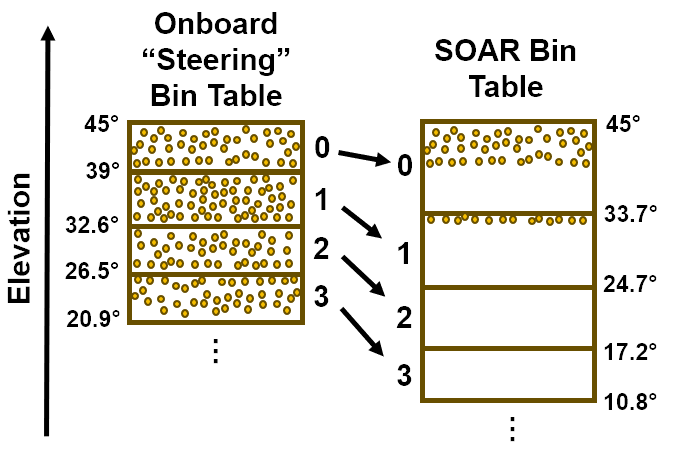
\includegraphics[width=0.75\linewidth]{figures/bin issue cartoon.png}
    \caption{A cartoon to illustrate the process by which a discrepancy in the two elevation binning tables used by SWA DPU can lead to incorrect elevation binning. The vertical axis indicates the elevation angle corresponding to various electron detections, which are represented by yellow circles. The first four bins for the two binning tables are represented by rectangles labelled with their indices and the angles of their upper and lower elevation bounds, and vertically scaled according to their elevation widths. The short arrows indicate the correspondence between the indices of the mismatched binning tables.}
    \caption*{Image Source: Author's own work}
    \label{fig: bin issue cartoon}
\end{figure}

\newpage
\section{Completeness Algorithm} \label{completeness}
Research into the steering algorithm and data visualisation completed earlier in this project made it clear that there is a relatively fast approach to generating a \q{completeness} or \q{quality} score for Burst Mode PADs, circumventing the relatively expensive process of re-binning EAS Burst Mode VDF data to generate the PADs in the first place, and then assessing PAD completeness \q{by hand} (e.g. by counting the white bins in Figure \ref{fig: PAD example}).
\\

As previously described, while discrepancies between \(B_{EAS}\) and \(B_{MAG}\) are expected to cause some inaccuracies in Burst Mode PADs, the resulting PADs will only be left \textit{incomplete} if these discrepancies disrupt Burst Mode steering. That is, under otherwise-ideal conditions, in order to lose part of a \([0\degree-180\degree)\) distribution, not only must \(B_{EAS}\) lie within a different angular bin than \(B_{MAG}\), but, more specifically, it must lie within a different \textit{elevation} bin than the actual bin(s) selected. Differences in azimuthal bin selection would lead the pitch angles recovered from the azimuthal bins in each selected elevation band (e.g. as shown in Figure \ref{fig: normal - full contours + selection}) to be labelled incorrectly, but this can be corrected in post-processing as long as \(B_{MAG}\) is known. No amount of re-labelling can recover a pitch angle that would have fallen within an elevation bin that was not sampled. The exact amount of pitch angle \q{loss} therefore only depends on the elevation angles of \(B_{MAG}\) and the selected elevation bins. Consider the vector parallel to \(B_{EAS}\), whose selected elevation bin is meant to capture a range of pitch angles from 0\degree\ (for the pixel containing the vector) to \(\geq90\degree\) (for the pixel in the same elevation bin with \(+180\degree\) azimuth compared to the vector). If \(B_{MAG}\) lies outside of this elevation bin, then, after re-labelling pitch angle data, the smallest pitch angle that can be recovered is theoretically equal to the smallest difference in elevation between \(B_{MAG}\) and each of the two boundaries (upper and lower) of the selected parallel elevation bin. Any electron with a pitch angle smaller than this difference is travelling too close to parallel with \(B_{MAG}\) to be captured by the selected elevation bin and therefore goes undetected. More formally, let \(B_{EAS, \ppara}\), \(B_{EAS, \apara}\), \(B_{MAG, \ppara}\), and \(B_{MAG, \apara}\) represent the unit vectors parallel and anti-parallel to \(B_{EAS}\) and \(B_{MAG}\) respectively. Working in the selected EAS head frame, the pitch angle loss \(\Delta_{\ppara}\) associated with \(B_{EAS, \ppara}\) is given by:

\begin{equation} \label{eq: parallel loss}
    \Delta_{\ppara}=\min\{|\theta_{MAG, \ppara}-\theta_{upper, \ppara}|, |\theta_{MAG, \ppara}-\theta_{lower, \ppara}|\}
\end{equation}

where \(\theta_{MAG, \ppara}\) is the elevation of \(B_{MAG, \ppara}\) and \(\theta_{upper, \ppara}\) and \(\theta_{lower, \ppara}\) are the elevations of the upper and lower boundaries of the selected parallel elevation bin respectively. \(\Delta_{\ppara}\) is equivalent to the minimum theoretical pitch angle \(\alpha_{min}\) that can be recovered from a Burst Mode PAD, yielding the identity:

\begin{equation} \label{eq: alpha min}
    \alpha_{min}=\Delta_{\ppara}
\end{equation}

Similarly, the pitch angle loss \(\Delta_{\apara}\) associated with \(B_{EAS, \apara}\) is given by:

\begin{equation} \label{eq: antiparallel loss}
    \Delta_{\apara}=\min\{|\theta_{MAG, \apara}-\theta_{upper, \apara}|, |\theta_{MAG, \apara}-\theta_{lower, \apara}|\}
\end{equation}

where \(\theta_{MAG, \apara}\) is the elevation of \(B_{MAG, \apara}\) and \(\theta_{upper, \apara}\) and \(\theta_{lower, \apara}\) are the elevations of the upper and lower boundaries of the selected anti-parallel elevation bin respectively. As before, \(\Delta_{\apara}\) implies that any electrons with a pitch angle larger than a maximum theoretical pitch angle \(\alpha_{max}\) cannot be detected. Therefore, if all angles are expressed in degrees, then the maximum theoretical pitch angle that can be recovered from a Burst Mode PAD is given by:

\begin{equation} \label{eq: alpha max}
    \alpha_{max}=180\degree-\Delta_{\apara}
\end{equation}

Notably, the fact that pitch angle loss occurs first at an \(\alpha_{min}\) and \(\alpha_{max}\) at either end of a full PAD before \q{spreading} towards the center of the distribution may imply that EAS Burst Mode is particularly ineffective at capturing narrow electron strahl populations in the solar wind, which are aligned with \(B_{MAG, \ppara}\) or \(B_{MAG, \apara}\) by definition\cite{kajdic2016}.
\\

In general, it should \textit{not} be assumed that \(\Delta_{\ppara}=\Delta_{\apara}\) because the specific elevation bins associated with \(B_{EAS, \ppara}\) and \(B_{EAS, \apara}\) are calculated independently of each other and, in general, the elevation bins for both sensor heads are of non-uniform width\cite{owen2020}\cite{owen2021}. In other words, a loss of \(\Delta_{\ppara}\) with respect to the parallel bin does \textit{not} imply a symmetric and equal loss \(\Delta_{\apara}\) with respect to the anti-parallel bin. This asymmetry can be captured using the visualisation tool described in Section \ref{visualisation}. Using pre-existing code for plotting pitch angle contours, \(\alpha_{min}\) and \(\alpha_{max}\) can be treated as any other pitch angle and visualised in the same way as the pitch angles in Figures \ref{fig: normal - full contours} and Figure \ref{fig: normal - full contours + selection}. When \(\alpha_{min}\) and \(\alpha_{max}\) are visualised this way, the sizes (or \q{radii}) of their contours around \(B_{MAG, \ppara}\) and \(B_{MAG, \apara}\) on the plot represent the sizes of the losses \(\Delta_{\ppara}\) and \(\Delta_{\apara}\) respectively.  Using the period of Burst Mode data from 12th June 2023 as an example, \(\alpha_{min}\) and \(\alpha_{max}\) are presented in Figure \ref{fig: full contours + selection + loss} as pitch angle contours plotted in red around \(B_{EAS, \ppara}\) (the green diamond) and \(B_{EAS, \apara}\) (the green square) respectively. In this example, \(\alpha_{min}\) and \(\alpha_{max}\) (and, by extension, \(\Delta_{\ppara}\) and \(\Delta_{\apara}\)) are of visibly different sizes.
\\

\begin{figure}[h!]
    \centering
    \centerfloat
    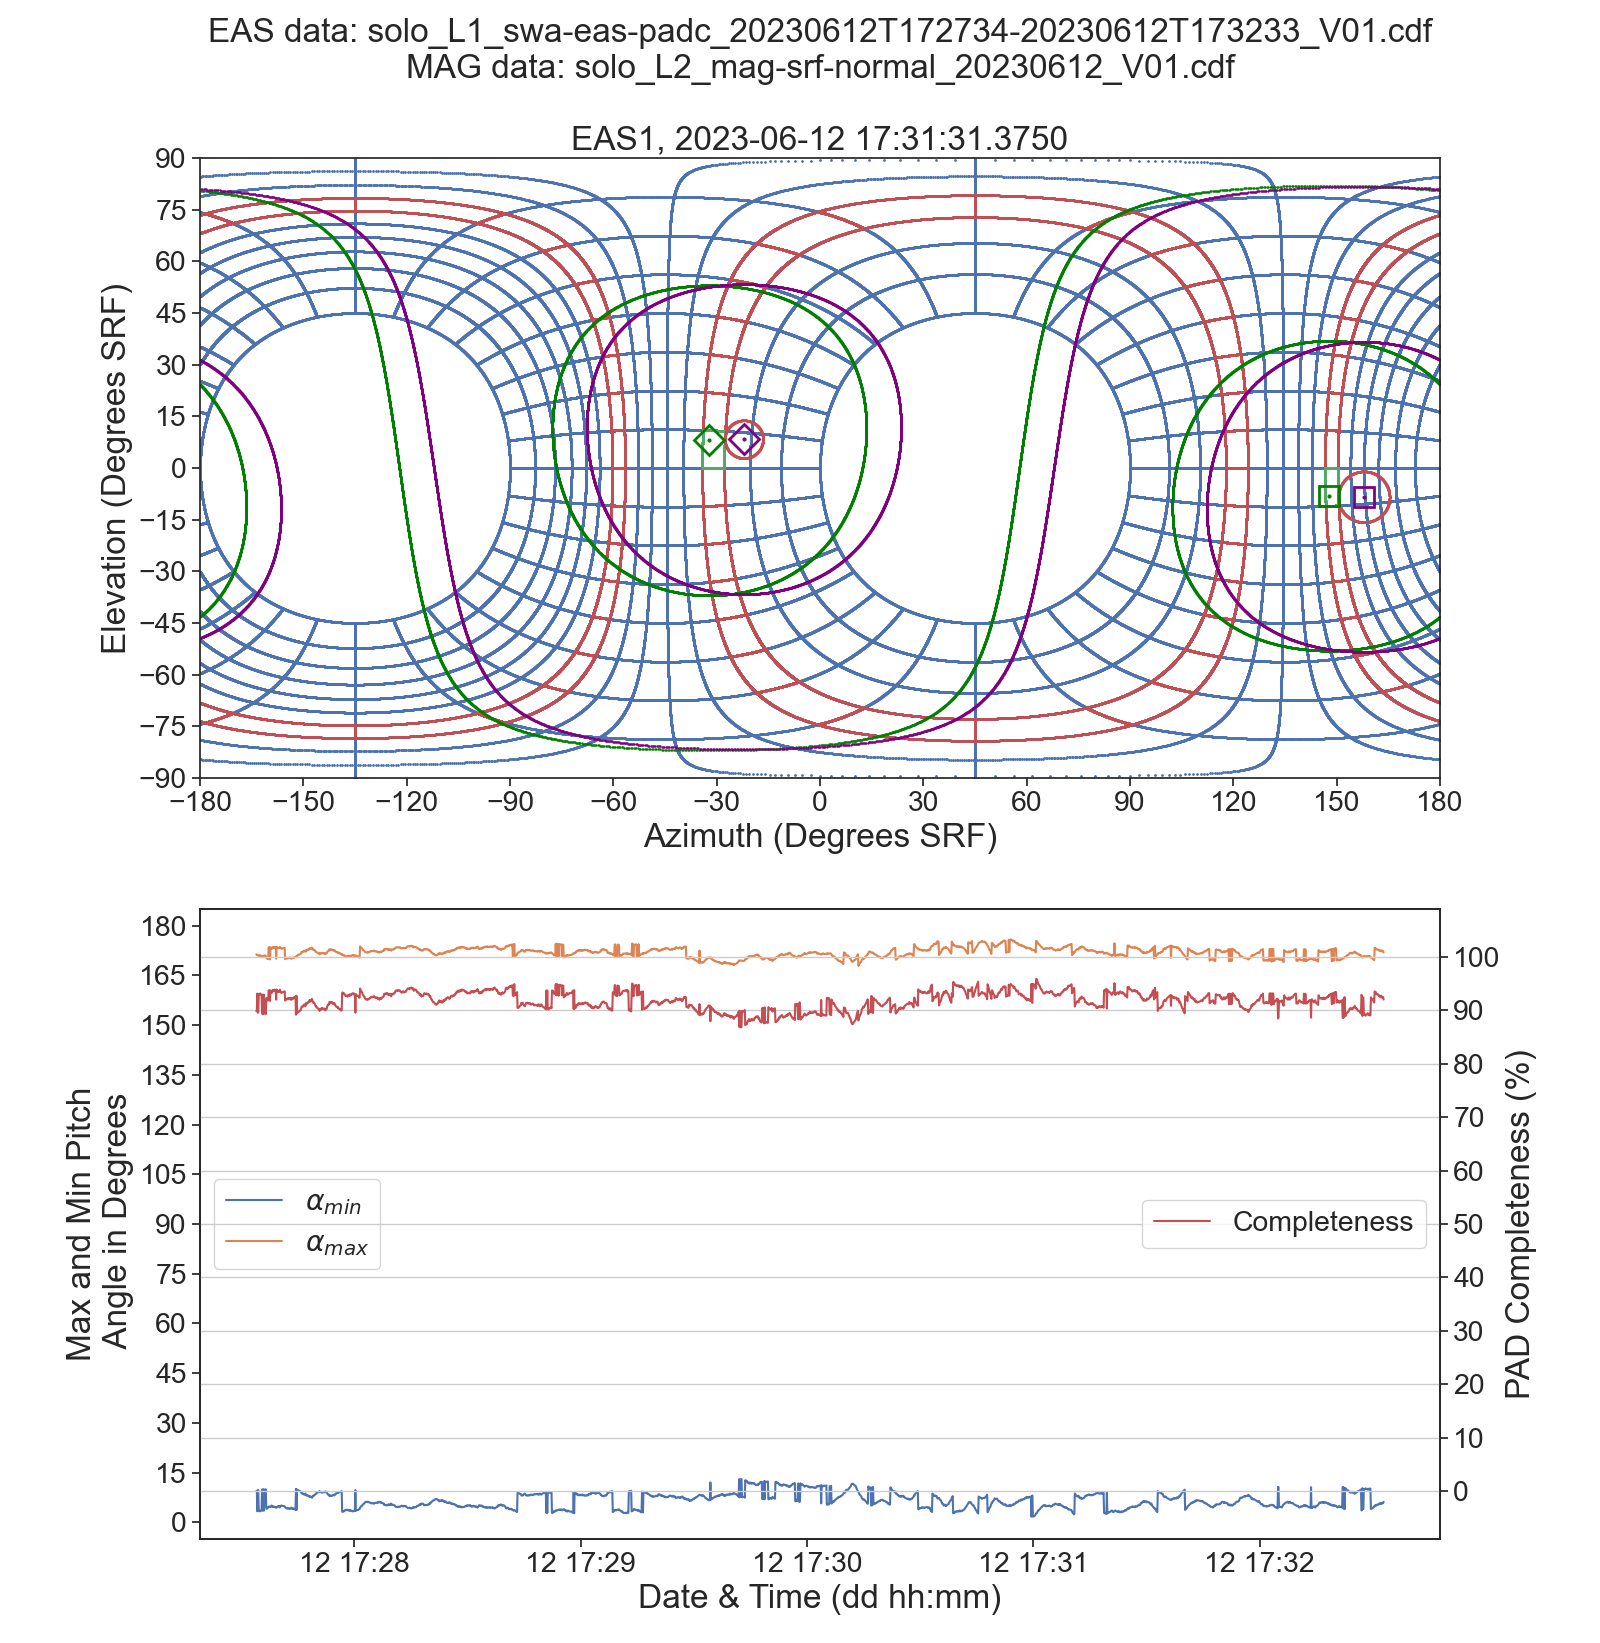
\includegraphics[width=1.2\linewidth]{figures/Verbose Example 12062023.png}
    \caption{Top panel: A plot of magnetic field vectors and calculated bin selection from 12th June 2023. Diamond and square markers represent parallel and anti-parallel magnetic field vectors respectively. Green represents \Beas\ and purple represents \Bmag. \(\alpha_{min}\) and \(\alpha_{max}\) are plotted as contours in red. Bottom panel: A plot of min and max pitch angles \(\alpha_{min}\) and \(\alpha_{max}\) and PAD completeness \textit{C} over the same period. \(\alpha_{min}\) and \(\alpha_{max}\) are plotted on the angular axis on the left, and \textit{C} is plotted on the percentage axis on the right.}
    \caption*{Image Source: Author's own work}
    \label{fig: full contours + selection + loss}
\end{figure}

The total angular loss in a Burst Mode PAD depends on the combined contributions of the parallel and anti-parallel losses \(\Delta_{\ppara}\) and \(\Delta_{\apara}\). Subtracting the total loss from the full \([0\degree-180\degree]\) range of an ideal PAD with lossless binning and steering gives the widest theoretical range of pitch angles that can be captured by that PAD. Taking the size of that range as a fraction of a full 180\degree\ yields the following metric of the PAD's completeness \textit{C}, where all angles are expressed in degrees:

\begin{equation} \label{eq: completeness}
    C=\frac{180\degree-\Delta_{\apara}-\Delta_{\ppara}}{180\degree}=\frac{\alpha_{max}-\alpha_{min}}{180\degree}
\end{equation}

\newpage
In summary, an algorithm for calculating the completeness of a Burst Mode PAD at a particular point in time \textit{t} can be described as follows:
\begin{enumerate} \label{alg: C algorithm}
    \item Acquire the upper and lower boundaries of the parallel and anti-parallel elevation bins selected by SWA-DPU at \textit{t}. In terms of the variables in SOAR EAS L1 \textit{.cdf} files, these boundaries can be calculated by summing the vectors from \q{SWA\_EAS\_ELEVATION} and \q{SWA\_EAS\_ELEVATION\_delta\_upper},  and from \q{SWA\_EAS\_ELEVATION} and \q{SWA\_EAS\_ELEVATION\_delta\_lower} at \textit{t} respectively.

    \item Acquire the EAS sensor head selected by SWA-DPU at \textit{t}. In terms of the variables in SOAR EAS L1 \textit{.cdf} files, these can be found under \q{SWA\_EAS\_EasUsed}.
    
    \item Identify the 8Hz MAG dataset containing the contemporaneous \Bmag\ vector at \textit{t}, and acquire the parallel and anti-parallel \Bmag\ vectors for that time. For simplicity, this dataset should be chosen such that the \Bmag\ vectors are already in cartesian SRF coordinates (see Section \ref{data}).

    \item Using the transformation matrices in the right column of Table \ref{tab: EASX to SRF}, transform the parallel and anti-parallel \Bmag\ vectors from cartesian SRF coordinates to the cartesian coordinates of the EAS sensor head selected at \textit{t} (\q{EASX}).

    \item Transform the parallel and anti-parallel \Bmag\ vectors from cartesian EASX coordinates to spherical EASX coordinates, and acquire their elevation angles in the range \([-90\degree,+90\degree]\)\footnote{Even though each EAS head can only sample the elevation range \([-45\degree,+45\degree]\), \Bmag\ vectors are not prevented from having an elevation outside of that range.}. 

    \item For each of the parallel and anti-parallel \Bmag\ vectors, check if their elevation angles are correctly binned by checking if they are between the upper and lower selected elevation bin boundaries. If either one is already correctly binned, then its associated loss is zero. 

    \item For each vector that is not already correctly binned, calculate the difference between its elevation and the elevation of the upper and lower selected elevation bin boundaries. The smallest of those two differences represents \(\Delta_{\ppara}\) for the parallel \Bmag\ vector or \(\Delta_{\apara}\) for the anti-parallel \Bmag\ vector.

    \item Use \(\Delta_{\ppara}\) and \(\Delta_{\apara}\) to calculate \textit{C} at \textit{t} according to Equation \ref{eq: completeness}.
\end{enumerate}
\\

\noindent This algorithm is relatively inexpensive to compute when compared to an alternative approach where EAS L1 data are completely re-binned into an accurate PAD and the missing pitch angle bins are counted manually. This is an algorithm that could be computed shortly after the receipt of EAS L1 data on the condition that contemporaneous MAG data are also downlinked and post-processed on the ground in a timely manner. Furthermore, the convenience of expressing PAD completeness as a single number, \textit{C}, may allow for faster determination of useful/unusable PADs for specific research purposes. For example, when investigating narrow, field-aligned electron strahl populations, high-\textit{C} may be a necessity to avoid missing all or most of the beams being studied. On the other hand, PADs with very low \textit{C} might be expected to have a limited range of pitch angle measurements, but multiple measurements of the same pitch few angles at varying gyrophase angles. Repeated measurements of the same pitch angle are redundant under the assumption of gyrotropy, but 8Hz measurements of gyrophase may provide a way to test that assumption using science data that are already available on SOAR, which \textit{C} could be used to identify\cite{owen2021}.
\\

While \textit{C} represents the theoretical maximum fraction of pitch angles available in a PAD, the effective range also depends on the choice of pitch angle binning. When EAS Burst Mode was introduced by Owen et al (2021), it was proposed that EAS VDFs could be resampled into eighteen 10\degree-wide pitch angle bins (this can be seen in the example in Figure \ref{fig: PAD example})\cite{owen2021}. If this number of bins is kept constant, then pitch angle loss would cause the bins at either end of the distribution either not to be \q{filled} or to be completely empty; their own form of incompleteness. Incomplete bins, if not completely discarded, should be analysed with caution as they may lead to misleading conclusions about the true electron PAD. Another approach is to vary the bin width, uniformly or non-uniformly, to maximise the actual range of pitch angles that can be analysed. In large datasets with varying completeness, the range of usable pitch angles may have to be sacrificed for the convenience of using standardised bin widths and bin numbers.
\\

So far, only the discrepancy between \(B_{EAS}\) and \(B_{MAG}\) has been examined for its effect on PAD completeness. However, the binning issue described in Section \ref{sim steering} should be expected to have its own effects on PAD completeness. Luckily, these effects are expected to be completely captured by the completeness algorithm. The binning issue concerns the discrepancy between \(B_{EAS}\) and its selected elevation bins, while the completeness algorithm concerns the discrepancy between \(B_{MAG}\) and the selected elevation bins. Whether or not these elevation bins were selected correctly for \(B_{EAS}\) only affects the completeness score indirectly depending on the agreement between \(B_{EAS}\) and \(B_{MAG}\). In fact, given sufficient disagreement between \(B_{EAS}\) and \(B_{MAG}\), the binning issue may lead \(B_{MAG}\) to be binned \textit{more accurately} than \(B_{EAS}\) (for example, if \(B_{EAS}\) lies outside the selected bin while \(B_{MAG}\), by chance, lies inside the selected bin).
\\

In Figure \ref{fig: full contours + selection + loss}, \(\alpha_{min}\) and \(\alpha_{max}\) have been calculated using binning according to the 17th July 2021 bin tables from SOAR (see Appendix \ref{appendixlabel1}). The binning issue described in Section \ref{sim steering} makes this calculation inaccurate. By extension, Figure \ref{fig: full contours + selection + loss} is also inaccurate. A more accurate figure can be generated by calculating \(\alpha_{min}\) and \(\alpha_{max}\) with the actual bins selected. The result of reproducing Figure \ref{fig: full contours + selection + loss} with this \q{corrected} approach is Figure \ref{fig: full contours + REAL selection + loss}. By comparing Figure \ref{fig: full contours + selection + loss} and Figure \ref{fig: full contours + REAL selection + loss}, it can be seen that \(\alpha_{min}\) is significantly higher in the latter plot (\(\sim15\degree\)) than in the former plot (\(\sim5\degree\)), meaning that \(\Delta_{\ppara}\) is larger as a consequence of the wrongly-selected elevation bin being farther from both \(B_{EAS, \ppara}\) and \(B_{MAG, \ppara}\). In contrast, it can also be seen that \(\alpha_{max}\) is somewhat higher in the latter plot (\(\sim175\degree\)) than in the former plot (\(\sim170\degree\)), meaning that \(\Delta_{\apara}\) is \textit{smaller} as a consequence of the wrongly-selected elevation bin being farther from \(B_{EAS, \apara}\) but closer to \(B_{MAG, \apara}\) by coincidence.
\\

\begin{figure}[h!]
    \centering
    \centerfloat
    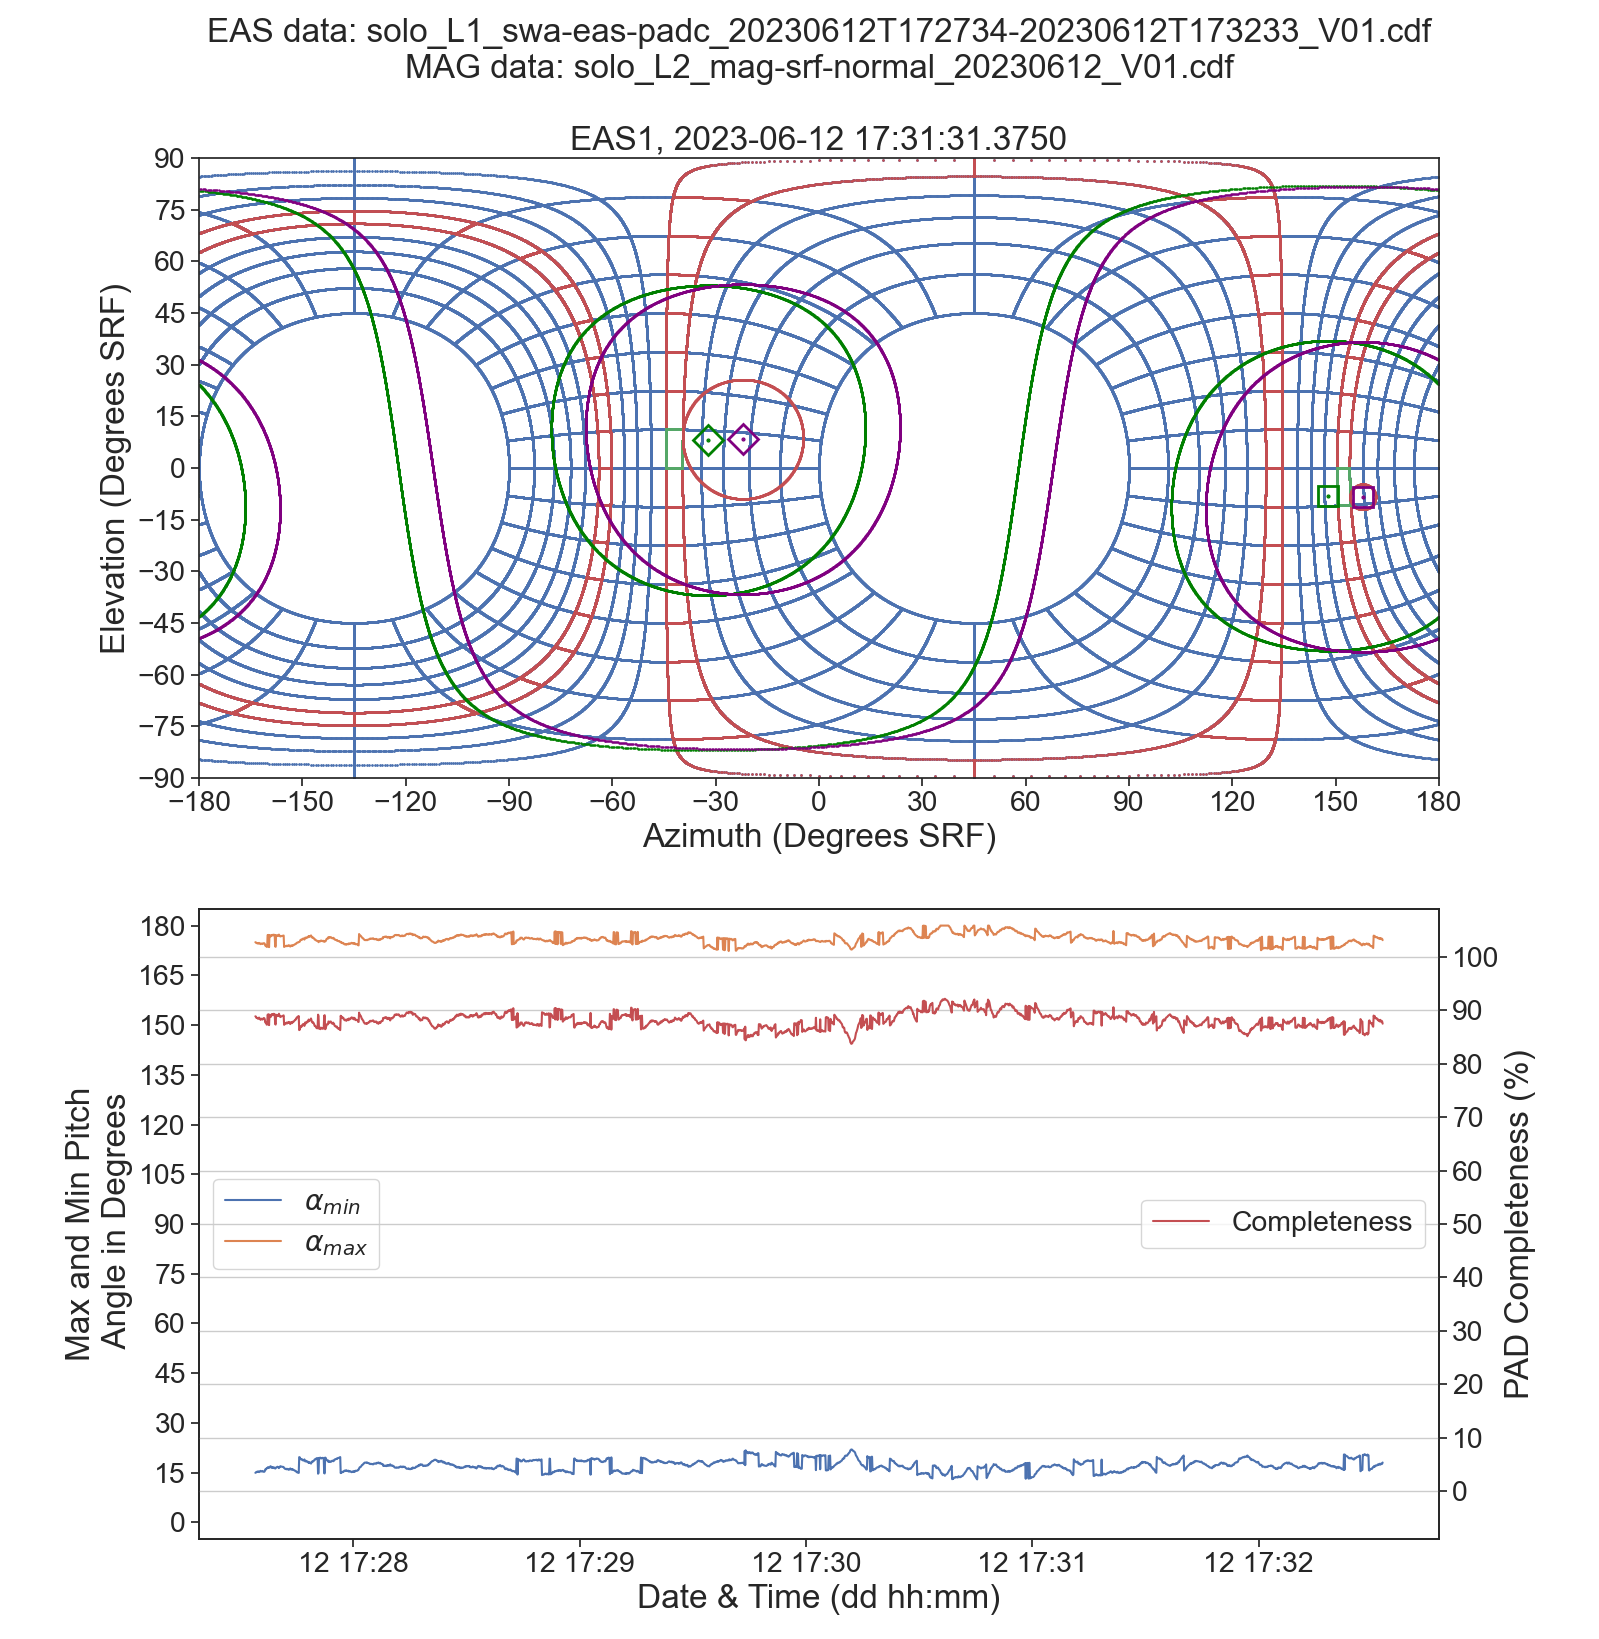
\includegraphics[width=1.2\linewidth]{figures/Verbose Example 12062023 Real.png}
    \caption{Top panel: A plot of magnetic field vectors and bin selection from 12th June 2023, where the binning issue is visible. Diamond and square markers represent parallel and anti-parallel magnetic field vectors respectively. Green represents \Beas\ and purple represents \Bmag. \(\alpha_{min}\) and \(\alpha_{max}\) are plotted as contours in red. Bottom panel: A plot of min and max pitch angles \(\alpha_{min}\) and \(\alpha_{max}\) and PAD completeness \textit{C} over the same period. \(\alpha_{min}\) and \(\alpha_{max}\) are plotted on the angular axis on the left, and \textit{C} is plotted on the percentage axis on the right.}
    \caption*{Image Source: Author's own work}
    \label{fig: full contours + REAL selection + loss}
\end{figure}

Equation \ref{eq: completeness} assumes the use of a basic VDF re-binning pipeline where pitch angles in the range \([0\degree,>90\degree]\) are re-binned from the parallel selected elevation bin and pitch angles in the range \([<90\degree,180\degree]\) are re-binned from the anti-parallel selected elevation bin. However, with sufficient disagreement between \(B_{EAS}\) and \(B_{MAG}\), it is theoretically possible for \(B_{MAG, \ppara}\) to be closer to either boundary of the \textit{anti}-parallel selected elevation bin than it is to the parallel selected elevation bin. Therefore, in that scenario, there may be a theoretical reduction in loss if the pitch angles in the range \([0\degree,>90\degree]\) were re-binned from the \textit{anti}-parallel selected elevation bin instead of the parallel selected elevation bin. This scenario is particularly likely if \(B_{EAS}\) is close to the selected EAS head's aperture center plane, because this should cause EAS to select parallel and anti-parallel elevation bins that are close to each other. An example of this phenomenon is found in Burst Mode data from 1st January 2023, and is shown in Figure \ref{fig: para antipara crossover} along with contours for \(\alpha_{min}\) and \(\alpha_{max}\) as calculated using Equations \ref{eq: alpha min} and \ref{eq: alpha max} respectively. In Figure \ref{fig: para antipara crossover}, the two selected elevation bins are adjacent to each other, and \(B_{MAG, \ppara}\) lies inside a different elevation bin than \(B_{EAS, \ppara}\). Although \(\alpha_{min}\) is still calculated and plotted under the assumption that it will be recovered from the parallel elevation bin, it is possible that \(\alpha_{min}\) (and therefore \(\Delta_{\ppara}\)) could be eliminated entirely if the anti-parallel elevation bin, in which \(B_{MAG, \ppara}\) lies, was used instead.
\\

This alternative approach would imply alternative calculations for the loss, yielding \(\Delta_{alt, \ppara}\) and \(\Delta_{alt, \apara}\), which are given by Equations \ref{eq: loss para _alt} and \ref{eq: loss anti _alt}.  These equations differ from Equations \ref{eq: parallel loss} and \ref{eq: antiparallel loss} in that \(\theta_{MAG, \ppara}\) and \(\theta_{MAG, \apara}\) are each compared to the elevations of \textit{all four} boundaries across both selected elevation bins instead of considering only the two boundaries of a single bin. In this case, the loss is given by the minimum angular distance of all four comparisons. As shown in Equations \ref{eq: loss para _alt} and \ref{eq: loss anti _alt}, this can be expressed succinctly by substituting \(\Delta_{\ppara}\) and \(\Delta_{\apara}\) for their equivalent expressions in Equations \ref{eq: parallel loss} and \ref{eq: antiparallel loss}.

\begin{equation} \label{eq: loss para _alt}
    \Delta_{alt, \ppara}=\min\{\Delta_{\ppara}, |\theta_{MAG, \ppara}-\theta_{upper, \apara}|, |\theta_{MAG, \ppara}-\theta_{lower, \apara}|\}
\end{equation}

\begin{equation} \label{eq: loss anti _alt}
    \Delta_{alt, \apara}=\min\{\Delta_{\apara}, |\theta_{MAG, \apara}-\theta_{upper, \ppara}|, |\theta_{MAG, \apara}-\theta_{lower, \ppara}|\}
\end{equation}

An equivalent completeness score \(C_{alt}\), is given by:

\begin{equation} \label{eq: C_alt}
    C_{alt}=\frac{180\degree-\Delta_{alt, \apara}-\Delta_{alt, \ppara}}{180\degree}
\end{equation}

\(C_{alt}\) can be incorporated into the algorithm for calculating \(C\) presented on page \pageref{alg: C algorithm} by changing steps 6 and 7 to require both the parallel and anti-parallel selected bins to be checked and compared against the \Bmag\ vector, and by changing step 8 to use Equation \ref{eq: C_alt}.
\\

\begin{figure}[h!]
    \centering
    \centerfloat
    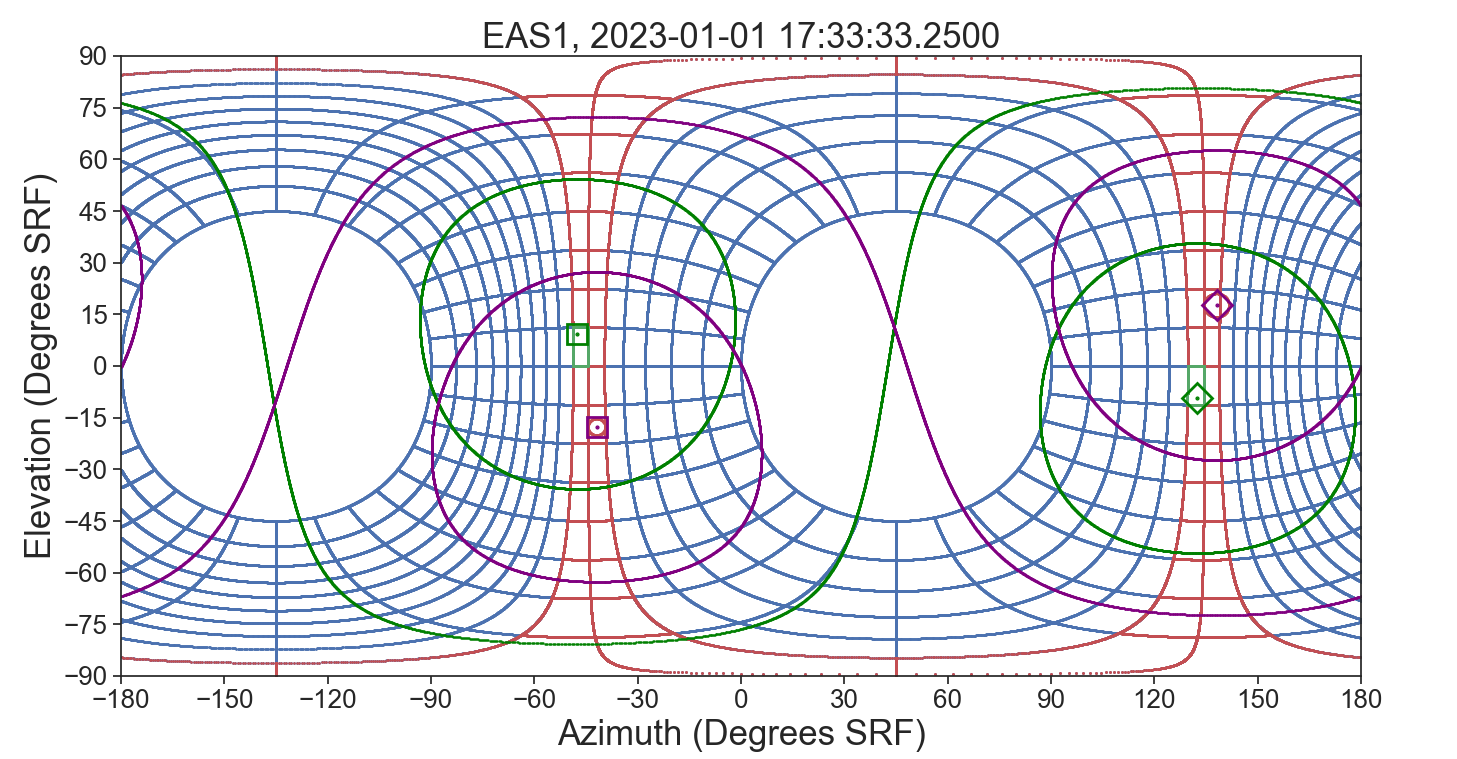
\includegraphics[width=1.1\linewidth]{figures/Crossover Example.png}
    \caption{A plot of magnetic field vectors and calculated bin selection from 1st January 2023, where the parallel and anti-parallel elevation bins are adjacent to each other. Diamond and square markers represent parallel and anti-parallel magnetic field vectors respectively. Green represents \Beas\ and purple represents \Bmag. \(\alpha_{min}\) and \(\alpha_{max}\) are plotted as (barely visible) contours in red.}
    \caption*{Image Source: Author's own work}
    \label{fig: para antipara crossover}
\end{figure}


\noindent \(C\), \(C_{alt}\) and the algorithms used to calculate them represent two relatively inexpensive approaches to determining the completeness of any given Burst Mode PAD based only on data for the contemporaneous MAG vector used (\Bmag) and the EAS elevation bins selected. In particular, \(C\) and its associated losses and min/max pitch angles have been calculated and presented for various instances of randomly selected sample data in this report, but future work could investigate the long-term variation of \textit{C}, collating months or years of EAS Burst Mode data available from SOAR. This may reveal a relationship between completeness and the time elapsed since the last routine calibration update to correct MAG offset drift, or a relationship between completeness and the rate of change of the magnetic field, potentially driven by magnetic turbulence in the solar wind\cite{smith2021}. 

\newpage
\section{S20 Link Latency} \label{S20 Link Latency}

To test the S20 latency algorithm described in Section \ref{S20 method} using real magnetic field data, a sample of \Bmag\ data from 30th May 2023 was given a large, artificial time offset of 50s and cross-correlated with itself, yielding two versions of it to represent an equivalent of \(f(t)\) and \(g(t)\) as previously described. The result for the \Bmag\ elevation in EAS1 coordinates is presented in Figure \ref{fig: arti 50s}. Only a single axis is considered here to avoid having to combine different measurements of the time delay from different axes, as described in detail in the author's previous work\cite{dickson2024}. The precision here is surprisingly high, yielding \(\tau_r=49.9\textrm{s}\pm1.8\)s, and the error bar associated with this uncertainty is barely visible on the lower panel of Figure \ref{fig: arti 50s}. The algorithm was then applied again, with a shorter time delay of 5s, yielding Figure \ref{fig: arti 5s}. Surprisingly again, the precision in this case was also high, yielding \(\tau_r=4.90\textrm{s}\pm0.2\)s. If this trend in increasing precision continues, then the S20 latency algorithm may be able to accurately characterise real differences between \Bmag\ and \Beas\ data more effectively than the author's previous attempts\cite{dickson2024}. This is an exciting subject that warrants future investigation.

\begin{figure}[h!]
    \centering
    \centerfloat
    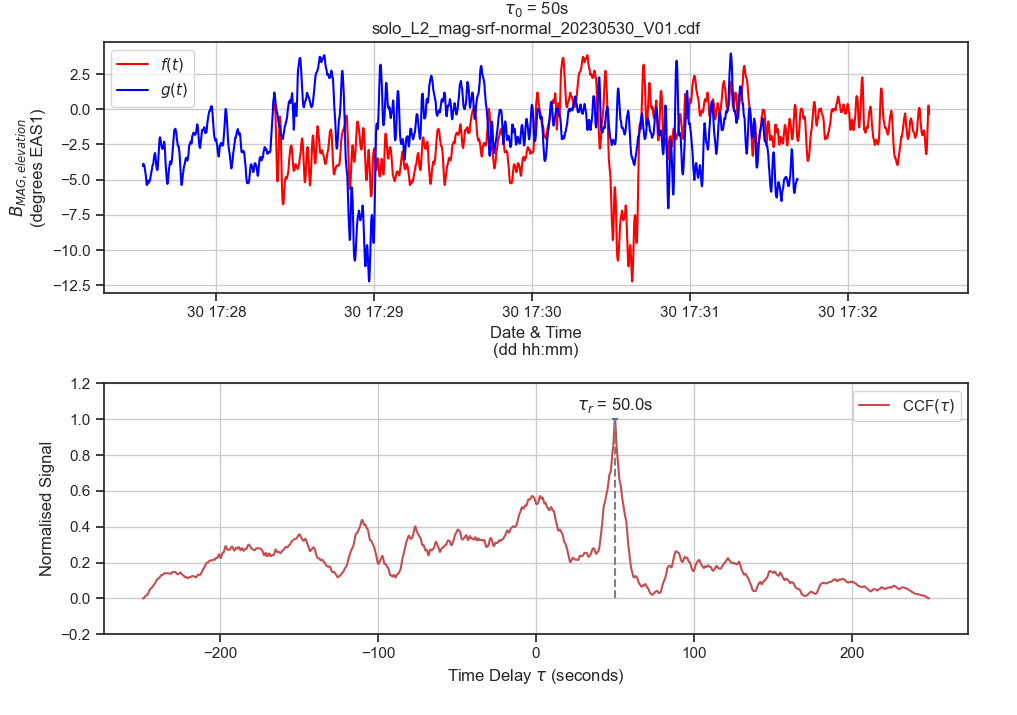
\includegraphics[width=1.3\linewidth]{figures/artificial delay 50s.png}
    \caption{Top panel: Two \q{identical} plots of \Beas\ elevation in EAS1 coordinates with an artificial, 50s time delay between them. Bottom panel: The result of the CCF algorithm applied to the top panel, where the uncertainty in \(\tau_r\) is indicated by the small, horizontal, blue bar.}
    \caption*{Image Source: Author's own work}
    \label{fig: arti 50s}
\end{figure}

\begin{figure}[h!]
    \centering
    \centerfloat
    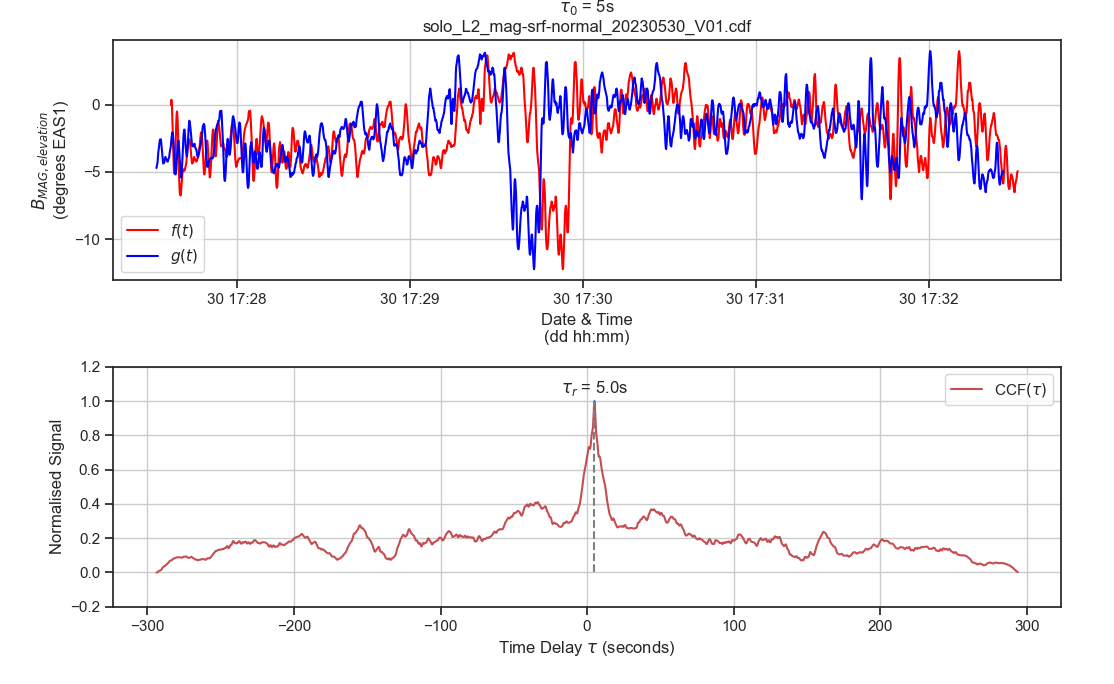
\includegraphics[width=1.35\linewidth]{figures/artificial delay 5s.png}
    \caption{Top panel: Two \q{identical} plots of \Beas\ elevation in EAS1 coordinates with an artificial, 5s time delay between them. Bottom panel: The result of the CCF algorithm applied to the top panel.}
    \caption*{Image Source: Author's own work}
    \label{fig: arti 5s}
\end{figure}
% \chapter{Discussion}
\label{chapterlabel6}

% This just dumps some pseudolatin in so you can see some text in place.
\blindtext
\chapter{Conclusion}
\label{chapterlabel4}
The goal of this project was to determine the accuracy and completeness of Solar Orbiter SWA-EAS Burst Mode PADs as a result of inaccuracies in \Beas\; the magnetic field vector data received by the SWA-DPU from MAG over the onboard S20 data link. These inaccuracies were expected to manifest as an offset between \Beas\ and \Bmag; the ground-processed magnetic field vector, and this was confirmed by preliminary comparisons between magnetic field time series performed using methodologies developed to crop and transform time series data acquired from the Solar Orbiter Archive. These offsets were found to be significant enough to lead to lost data in Burst Mode PADs, and this led to the development of an algorithm for \textit{C}; a concise metric for Burst Mode PAD completeness depending on pitch angle loss, represented by \(\Delta_{\ppara}\) and \(\Delta_{\apara}\). Pitch angle loss due to the inaccuracies described in this project manifests first near the extremities of a PAD at \(0\degree\) and \(180\degree\), which may have implications for future research investigating field-aligned electron strahl. Particularly high pitch angle loss (i.e. low PAD completeness) may also be valuable in its own right if it can be used to study agyrotropy. The metric \textit{C} can be a computationally inexpensive tool for classifying PAD data for any of these purposes.
\\

The development of \textit{C} was aided by the development of a tool for creating images and animations visualising EAS elevation-azimuth bins projected on to SRF coordinates along with time-varying magnetic field vectors, pitch angle contours, and PAD loss.
\\

One source of \Beas\ inaccuracy that this project aimed to investigate in particular was a possible latency over the S20 link. A method was developed to determine this latency by cross-correlation of \Beas\ and \Bmag\ using Monte Carlo error estimation, yielding promising, though inconclusive results.
\\

In addition to the project's primary goals, it also led to the discovery of some unexpected features in the EAS Burst Mode dataset. One such feature is a recurring issue with purported 8Hz \Beas\ data that is only updated at a 1Hz cadence, which may have consequences for Burst Mode data accuracy. Much has been said about the error in SWA-DPU whose discovery led to the deletion of \(\sim6\) months of EAS data from SOAR.
\\

For future work, a clear direction would be to apply the methods developed in this project for calculating \textit{C} and S20 latency to much larger sets of EAS and MAG data and investigate how those quantities vary over months or years. Similar surveys might lead to other discoveries, such as the prevalence and/or origin of the 8Hz-1Hz data issue. There is also plenty of room for improvement of the time series cropping and S20 latency determination algorithms that were hurriedly developed over the course of this project.

\phantomsection
\addcontentsline{toc}{chapter}{Appendices}
% The \appendix command resets the chapter counter, and changes the chapter numbering scheme to capital letters.
% \chapter{Appendices}
\appendix
\chapter{EAS Angular Bin Tables}
\label{appendixlabel1}
Tables containing elevation and azimuth binning data for both EAS heads can be found in some \textit{.cdf} files uploaded to SOAR. The uploaded tables have changed over the years since Solar Orbiter's commissioning, and tables associated with data uploaded at any time between 17th July 2021 and the time of writing are included here.
\\

\q{EAS1/2 Bin Index} refers to the index for each bin. \q{EAS1/2 Bin Index} is only used for the azimuthal bin table, because this table is identical for EAS1 and EAS2. The elevation bin tables are different for Eas1 and EAS2, hence the distinction between \q{EAS1 Bin Index} and \q{EAS2 Bin Index}. \q{Bin Center} refers to the angle of the center of each bin. \q{Bin Upper Delta} and \q{Bin Lower Delta} refer to the angular differences between \q{Bin Center} and the upper and lower boundaries of each bin respectively.
\\




\begin{table}[h]
    \centering
    \centerfloat
    \begin{tabular}{cccc}
        \textbf{EAS1/2 Bin Index} & \textbf{Bin Center (\degree)} & \textbf{Bin Upper Delta (\degree)} & \textbf{Bin Lower Delta (\degree)}\\
        0 & 5.625 & 5.625 & 5.625\\
        1 & 16.875 & 5.625 & 5.625\\
        2 & 28.125 & 5.625 & 5.625\\
        3 & 39.375 & 5.625 & 5.625\\
        4 & 50.625 & 5.625 & 5.625\\
        5 & 61.875 & 5.625 & 5.625\\
        6 & 73.125 & 5.625 & 5.625\\
        7 & 84.375 & 5.625 & 5.625\\
        8 & 95.625 & 5.625 & 5.625\\
        9 & 106.875 & 5.625 & 5.625\\
        10 & 118.125 & 5.625 & 5.625\\
        11 & 129.375 & 5.625 & 5.625\\
        12 & 140.625 & 5.625 & 5.625\\
        13 & 151.875 & 5.625 & 5.625\\
        14 & 163.125 & 5.625 & 5.625\\
        15 & 174.375 & 5.625 & 5.625\\
        16 & 185.625 & 5.625 & 5.625\\
        17 & 196.875 & 5.625 & 5.625\\
        18 & 208.125 & 5.625 & 5.625\\
        19 & 219.375 & 5.625 & 5.625\\
        20 & 230.625 & 5.625 & 5.625\\
        21 & 241.875 & 5.625 & 5.625\\
        22 & 253.125 & 5.625 & 5.625\\
        23 & 264.375 & 5.625 & 5.625\\
        24 & 275.625 & 5.625 & 5.625\\
        25 & 286.875 & 5.625 & 5.625\\
        26 & 298.125 & 5.625 & 5.625\\
        27 & 309.375 & 5.625 & 5.625\\
        28 & 320.625 & 5.625 & 5.625\\
        29 & 331.875 & 5.625 & 5.625\\
        30 & 343.125 & 5.625 & 5.625\\
        31 & 354.375 & 5.625 & 5.625\\
    \end{tabular}
    \caption{Bin Table: EAS1/2 Azimuth (as found in SOAR) - 17th July 2021}
    \label{tab: Bin Table EAS Azimuth July 2021}
\end{table}

\begin{table}[h]
    \centering
    \centerfloat
    \begin{tabular}{cccc}
        \textbf{EAS1 Bin Index} & \textbf{Bin Center (\degree)} & \textbf{Bin Upper Delta (\degree)} & \textbf{Bin Lower Delta (\degree)}\\
        0 & 39.34 & 5.66 & 5.66\\
        1 & 29.17 & 4.514 & 4.514\\
        2 & 20.91 & 3.748 & 3.748\\
        3 & 13.98 & 3.179 & 3.179\\
        4 & 8.06 & 2.74 & 2.74\\
        5 & 2.91 & 2.409 & 2.409\\
        6 & -1.66 & 2.161 & 2.161\\
        7 & -5.82 & 1.996 & 1.996\\
        8 & -9.7 & 1.886 & 1.886\\
        9 & -13.43 & 1.841 & 1.841\\
        10 & -17.13 & 1.856 & 1.856\\
        11 & -20.94 & 1.95 & 1.95\\
        12 & -25.0 & 2.115 & 2.115\\
        13 & -29.53 & 2.413 & 2.413\\
        14 & -34.82 & 2.88 & 2.88\\
        15 & -41.36 & 3.655 & 3.655\\
    \end{tabular}
    \caption{Bin Table: EAS1 Elevation (as found in SOAR) - 17th July 2021}
    \label{tab: Bin Table EAS1 Elevation July 2021}
\end{table}

\begin{table}[h]
    \centering
    \centerfloat
    \begin{tabular}{cccc}
        \textbf{EAS2 Bin Index} & \textbf{Bin Center (\degree)} & \textbf{Bin Upper Delta (\degree)} & \textbf{Bin Lower Delta (\degree)}\\
        0 & 38.94 & 6.06 & 6.06\\
        1 & 28.25 & 4.633 & 4.633\\
        2 & 19.86 & 3.761 & 3.761\\
        3 & 12.99 & 3.111 & 3.111\\
        4 & 7.25 & 2.624 & 2.624\\
        5 & 2.35 & 2.272 & 2.272\\
        6 & -1.93 & 2.012 & 2.012\\
        7 & -5.78 & 1.838 & 1.838\\
        8 & -9.37 & 1.747 & 1.747\\
        9 & -12.84 & 1.722 & 1.722\\
        10 & -16.32 & 1.759 & 1.759\\
        11 & -19.97 & 1.887 & 1.887\\
        12 & -23.97 & 2.113 & 2.113\\
        13 & -28.57 & 2.485 & 2.485\\
        14 & -34.13 & 3.071 & 3.071\\
        15 & -41.1 & 3.897 & 3.897\\
    \end{tabular}
    \caption{Bin Table: EAS2 Elevation (as found in SOAR) - 17th July 2021}
    \label{tab: Bin Table EAS2 Elevation July 2021}
\end{table}

\chapter{Code Excerpts}
\label{appendixlabel2}

The full codebase for this project can be found in the author's GitHub repository: 

\textit{https://github.com/joratto/Solar-Orbiter-SWA-EAS-Data-Completeness-MSc}
\\

\lstset{basicstyle=\tiny, style=myCustomMatlabStyle}
\begin{lstlisting}[language=Python]
time_index = 0
for i in range(1,searchdivisions+1):
    time_index += int(length/2**i)*(time_array[time_index+int(length/2**i)] < time_reference)
while (time_array[time_index] < time_reference) and (time_index < length-1):
    time_index += 1
\end{lstlisting}
\captionof{lstlisting}{\q{Time Axis Cropping Algorithm}}
\label{alg: fast time crop}

\bgroup\obeylines



\egroup

For the bin visualisation algorithm described in Section \ref{visualisation}, a single elevation bin can be defined by keeping the elevation angle of successive points constant (and equal to an upper/lower bound) while the azimuth phase angle is varied according to a defined angular point density, and vice versa for a single azimuth bin. Repeating this for the upper and lower edge of an elevation bin and an azimuth bin defines an elevation-azimuth pixel. Once defined, the points delineating each pixel can be projected to SRF space in spherical coordinates with the following sequence of transformations: Spherical EAS1/2 \(\rightarrow\) Cartesian EAS1/2 \(\rightarrow\) Cartesian SRF \(\rightarrow\) Spherical SRF. This pixel point plotting algorithm was implemented in Python as described in Appendix Listing \ref{alg: pix point plot}, where k\_az and k\_el represent integer numbers of azimuth and elevation phase angles along a single bin edge respectively. This algorithm double-counts edges shared between adjacent pixels, trading a linear amount of computational efficiency for some convenience in plotting individual pixels. Once the points are transformed to spherical SRF coordinates, their azimuth angles are converted from the range [-180,180] to the range [0,360] for uniformity with EAS azimuth conventions. Given sufficient point density (20/\degree\ works well), this results in the visually curved bins shown in Figure \ref{fig: all bins}. Another result of high point density is that this algorithm's many matrix multiplications for each point transformation lead to a computation time of several minutes for a single image. To save time, the algorithm was adapted to save the point coordinates for each pixel to .csv files in a directory under \q{bin\_projections\(\backslash\)EAS\textit{X}\(\backslash\)el\textit{Y}\(\backslash\)EAS\textit{X}\_el\textit{Y}\_az\textit{Z}.csv} where \textit{X} is the EAS head number and \textit{Y} and \textit{Z} are the elevation and azimuth bin indices respectively. These files can then be read and plotted with an order of magnitude reduction in computation time. Part of this algorithm's Python implementation is as shown in Appendix Listing \ref{alg: pix point save}.
\\

\lstset{basicstyle=\tiny, style=myCustomMatlabStyle}
\begin{lstlisting}[language=Python]
angleStep = 1/pointDensity
azimuthPointCount = int(pointDensity*360/azimBinCount)
for i in range(elevBinCount):
    elevationBinWidth = 2*elevDeltaLowerArray[i]
    elevationPointCount = int(point_density*elevationBinWidth)
    binBoundaryProjectionArray.append([])
    for j in range(azimBinCount):
        pointArray = []
        for k_az in range(0,azimuthPointCount):
            lowerEdge_elev = np.array([1, elevLowerBoundArray[i], azimLowerBoundArray[j]+k_az*angleStep])
            lowerEdge_elev = cartToSphere(cart_proj_tuple[head].dot(sphereToCart(lowerEdge_elev)))
            pointArray.append(lowerEdge_elev)

            upperEdge_elev = np.array([1, elevUpperBoundArray[i], azimLowerBoundArray[j]+k_az*angleStep])
            upperEdge_elev = cartToSphere(cart_proj_tuple[head].dot(sphereToCart(upperEdge_elev)))
            pointArray.append(upperEdge_elev)

        for k_el in range(0,elevationPointCount):
            lowerEdge_azim = np.array([1, elevLowerBoundArray[i]+k_el*angleStep, azimLowerBoundArray[j]])
            lowerEdge_azim = cartToSphere(cart_proj_tuple[head].dot(sphereToCart(lowerEdge_azim)))
            pointArray.append(lowerEdge_azim)

            upperEdge_azim = np.array([1, elevLowerBoundArray[i]+k_el*angleStep, azimUpperBoundArray[j]])
            upperEdge_azim = cartToSphere(cart_proj_tuple[head].dot(sphereToCart(upperEdge_azim)))
            pointArray.append(upperEdge_azim)
\end{lstlisting}
\captionof{lstlisting}{\q{Pixel Point Plotting Algorithm}}
\label{alg: pix point plot}

\lstset{basicstyle=\tiny, style=myCustomMatlabStyle}
\begin{lstlisting}[language=Python]
for i in range(16):
        for j in range(32):
                filename = 'bin_projections\EAS{head}\el{i}\EAS{head}_el{i}_az{j}.csv'
                pixelArray = np.genfromtxt(filename, delimiter=",")
                el = pixelArray[1]
                az = pixelArray[2]
                ax.scatter(az,el,color=bin_color,marker='.',s=s)
\end{lstlisting}
\captionof{lstlisting}{\q{Pixel Point Saving Algorithm}}
\label{alg: pix point save}

% (things)

\chapter{Colophon}
\label{appendixlabel3}
% \textit{This is a description of the tools you used to make your thesis. It helps people make future documents, reminds you, and looks good.}

% UCL Thesis LaTeX Template
%  (c) Ian Kirker, 2014
% 
% This is a template/skeleton for PhD/MPhil/MRes theses.

This document was set in the Times New Roman typeface using \LaTeX\ and Bib\TeX. It was composed using Overleaf. The document format is based on the \q{UCL Thesis \LaTeX\ Template} by Ian Kirker, which is available on GitHub\cite{kirker2014}. In addition, a few custom \LaTeX\ functions were used to make the writing process a bit easier. For example:
\\

\noindent Quotations are written using this function:
\begin{verbatim}
    \newcommand{\q}[1]{``#1''}
\end{verbatim}
The symbols \Beas\ and \Bmag\ are written using these functions:
\begin{verbatim}
    \newcommand{\Beas}{\(B_{EAS}\)}
    \newcommand{\Bmag}{\(B_{MAG}\)}
\end{verbatim}
The symbols \q{\(\ppara\)} and \q{\(\apara\)} are dependent on the \textit{amssymb} package for \LaTeX\ and are written using these functions: 
\begin{verbatim}
    \newcommand{\ppara}{\upharpoonleft \! \upharpoonright}
    \newcommand{\apara}{\upharpoonleft \! \downharpoonright}
\end{verbatim}
Large figures are occasionally plotted with a width \(>1\), which causes them to be un-centered on the page by default. The following function by \textit{tex.stackexchange.com} user Marc Baudoin keeps them centered\cite{baudoin2011}:
\begin{verbatim}
    \makeatletter
    \newcommand*{\centerfloat}{%
        \parindent \z@
        \leftskip \z@ \@plus 1fil \@minus \textwidth
         \rightskip\leftskip
        \parfillskip \z@skip}
    \makeatother
\end{verbatim}

\vspace*{\fill}
\noindent \q{I have made an end at last, and my weary hand can rest.}\cite{ruth2019}


 % description of document, e.g. type faces, TeX used, TeXmaker, packages and things used for figures. Like a computational details section.
% e.g. http://tex.stackexchange.com/questions/63468/what-is-best-way-to-mention-that-a-document-has-been-typeset-with-tex#63503

% Side note:
%http://tex.stackexchange.com/questions/1319/showcase-of-beautiful-typography-done-in-tex-friends
 
% You could separate these out into different files if you have
%  particularly large appendices.

% Actually generates your bibliography. The fact that \include is 
% the last thing before this ensures that it is on a clear page.
\bibliography{citations}

% All done. \o/
\end{document}
